% Created by tikzDevice version 0.9 on 2016-03-15 18:17:39
% !TEX encoding = UTF-8 Unicode
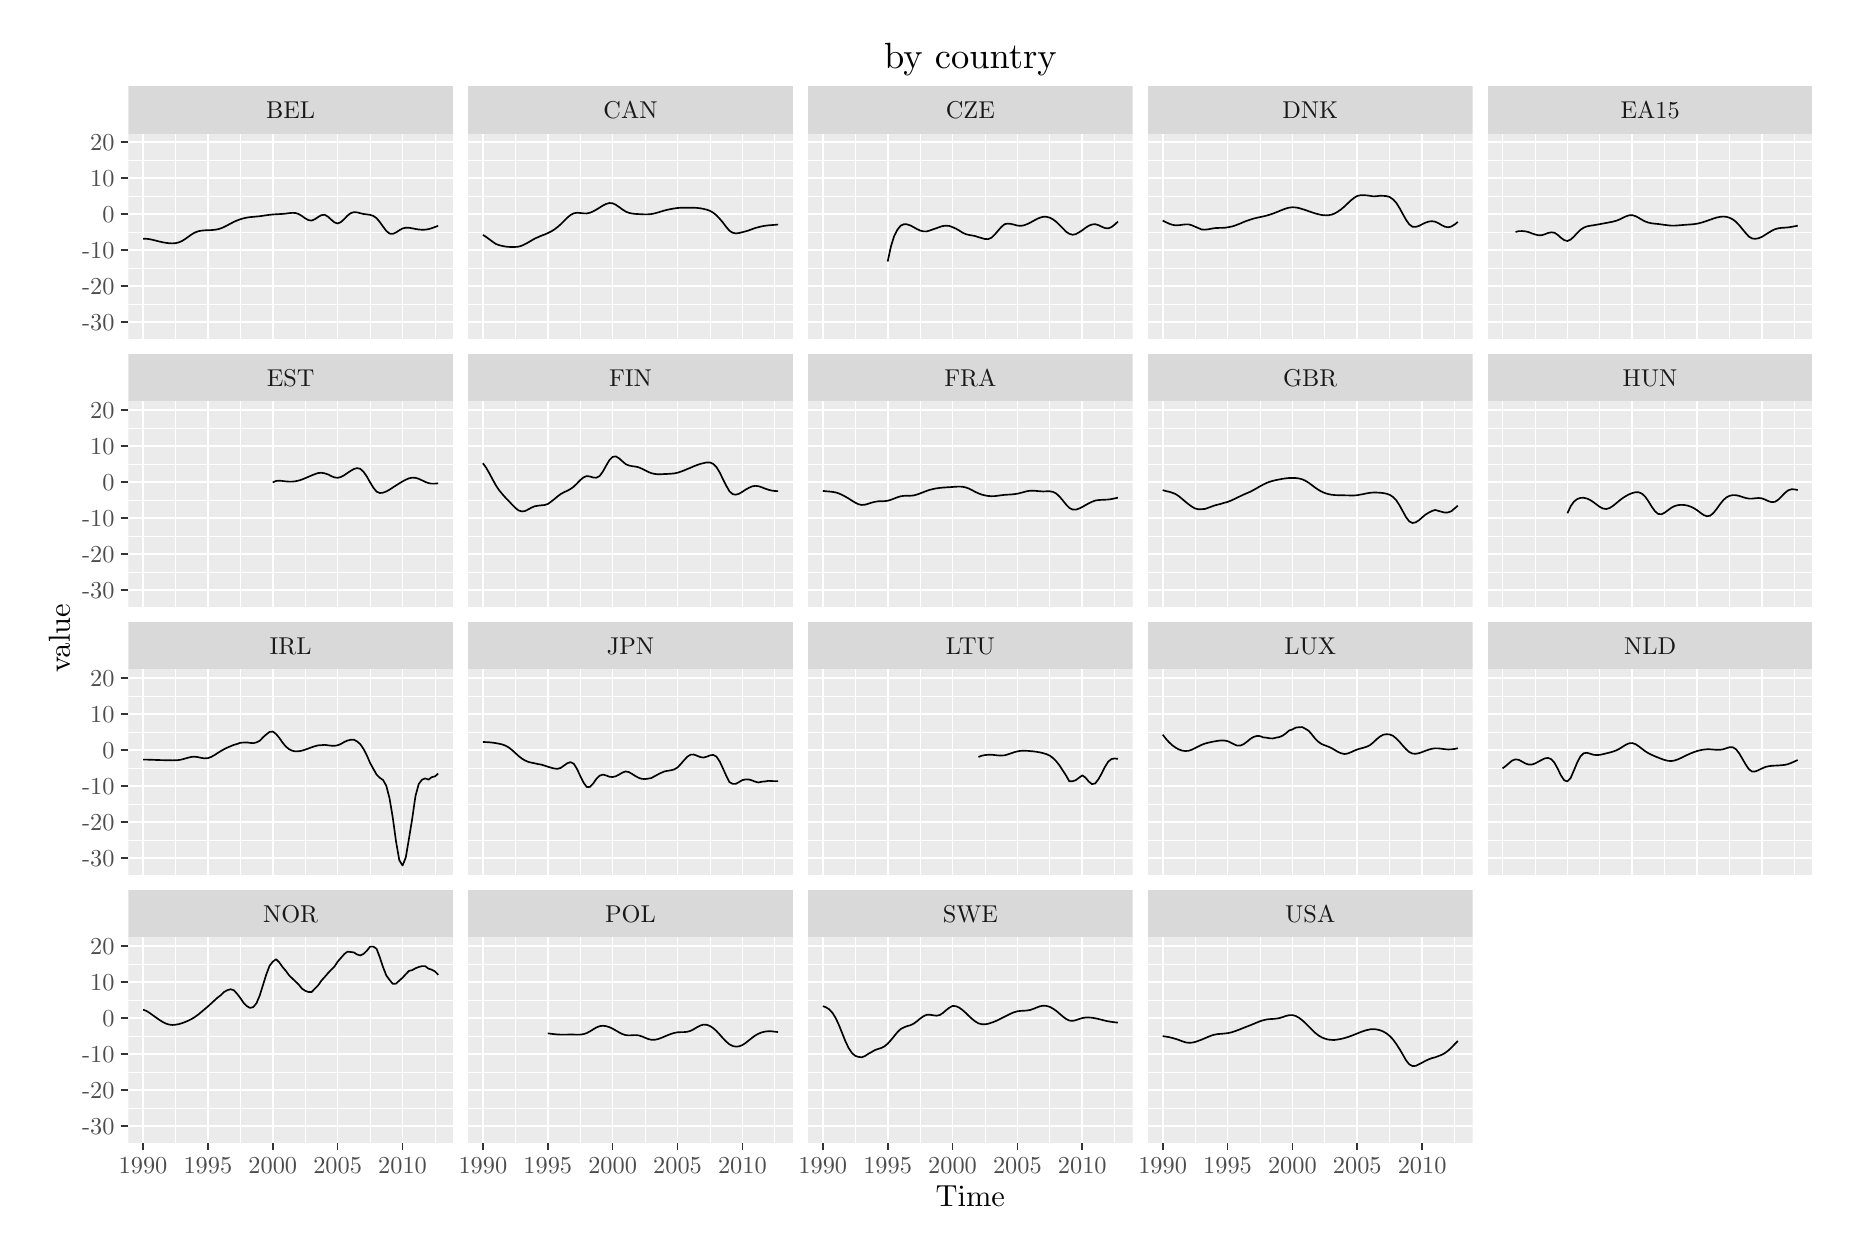
\begin{tikzpicture}[x=1pt,y=1pt]
\definecolor{fillColor}{RGB}{255,255,255}
\path[use as bounding box,fill=fillColor,fill opacity=0.00] (0,0) rectangle (650.43,433.62);
\begin{scope}
\path[clip] (  0.00,  0.00) rectangle (650.43,433.62);
\definecolor{drawColor}{RGB}{255,255,255}
\definecolor{fillColor}{RGB}{255,255,255}

\path[draw=drawColor,line width= 0.6pt,line join=round,line cap=round,fill=fillColor] (  0.00,  0.00) rectangle (650.43,433.62);
\end{scope}
\begin{scope}
\path[clip] ( 36.36,321.12) rectangle (153.67,395.37);
\definecolor{fillColor}{gray}{0.92}

\path[fill=fillColor] ( 36.36,321.12) rectangle (153.67,395.37);
\definecolor{drawColor}{RGB}{255,255,255}

\path[draw=drawColor,line width= 0.3pt,line join=round] ( 36.36,333.70) --
	(153.67,333.70);

\path[draw=drawColor,line width= 0.3pt,line join=round] ( 36.36,346.71) --
	(153.67,346.71);

\path[draw=drawColor,line width= 0.3pt,line join=round] ( 36.36,359.71) --
	(153.67,359.71);

\path[draw=drawColor,line width= 0.3pt,line join=round] ( 36.36,372.71) --
	(153.67,372.71);

\path[draw=drawColor,line width= 0.3pt,line join=round] ( 36.36,385.71) --
	(153.67,385.71);

\path[draw=drawColor,line width= 0.3pt,line join=round] ( 53.41,321.12) --
	( 53.41,395.37);

\path[draw=drawColor,line width= 0.3pt,line join=round] ( 76.85,321.12) --
	( 76.85,395.37);

\path[draw=drawColor,line width= 0.3pt,line join=round] (100.29,321.12) --
	(100.29,395.37);

\path[draw=drawColor,line width= 0.3pt,line join=round] (123.73,321.12) --
	(123.73,395.37);

\path[draw=drawColor,line width= 0.3pt,line join=round] (147.17,321.12) --
	(147.17,395.37);

\path[draw=drawColor,line width= 0.6pt,line join=round] ( 36.36,327.20) --
	(153.67,327.20);

\path[draw=drawColor,line width= 0.6pt,line join=round] ( 36.36,340.21) --
	(153.67,340.21);

\path[draw=drawColor,line width= 0.6pt,line join=round] ( 36.36,353.21) --
	(153.67,353.21);

\path[draw=drawColor,line width= 0.6pt,line join=round] ( 36.36,366.21) --
	(153.67,366.21);

\path[draw=drawColor,line width= 0.6pt,line join=round] ( 36.36,379.21) --
	(153.67,379.21);

\path[draw=drawColor,line width= 0.6pt,line join=round] ( 36.36,392.21) --
	(153.67,392.21);

\path[draw=drawColor,line width= 0.6pt,line join=round] ( 41.69,321.12) --
	( 41.69,395.37);

\path[draw=drawColor,line width= 0.6pt,line join=round] ( 65.13,321.12) --
	( 65.13,395.37);

\path[draw=drawColor,line width= 0.6pt,line join=round] ( 88.57,321.12) --
	( 88.57,395.37);

\path[draw=drawColor,line width= 0.6pt,line join=round] (112.01,321.12) --
	(112.01,395.37);

\path[draw=drawColor,line width= 0.6pt,line join=round] (135.45,321.12) --
	(135.45,395.37);
\definecolor{drawColor}{RGB}{0,0,0}

\path[draw=drawColor,line width= 0.6pt,line join=round] ( 41.69,357.33) --
	( 42.86,357.33) --
	( 44.03,357.19) --
	( 45.20,356.94) --
	( 46.38,356.65) --
	( 47.55,356.35) --
	( 48.72,356.08) --
	( 49.89,355.87) --
	( 51.06,355.72) --
	( 52.24,355.67) --
	( 53.41,355.75) --
	( 54.58,356.02) --
	( 55.75,356.52) --
	( 56.92,357.25) --
	( 58.10,358.10) --
	( 59.27,358.93) --
	( 60.44,359.61) --
	( 61.61,360.04) --
	( 62.78,360.27) --
	( 63.96,360.38) --
	( 65.13,360.43) --
	( 66.30,360.47) --
	( 67.47,360.57) --
	( 68.64,360.76) --
	( 69.82,361.10) --
	( 70.99,361.60) --
	( 72.16,362.20) --
	( 73.33,362.84) --
	( 74.50,363.44) --
	( 75.68,363.96) --
	( 76.85,364.39) --
	( 78.02,364.73) --
	( 79.19,364.98) --
	( 80.36,365.15) --
	( 81.54,365.27) --
	( 82.71,365.37) --
	( 83.88,365.49) --
	( 85.05,365.65) --
	( 86.22,365.82) --
	( 87.40,365.99) --
	( 88.57,366.11) --
	( 89.74,366.19) --
	( 90.91,366.25) --
	( 92.08,366.32) --
	( 93.26,366.43) --
	( 94.43,366.59) --
	( 95.60,366.70) --
	( 96.77,366.64) --
	( 97.94,366.27) --
	( 99.12,365.55) --
	(100.29,364.72) --
	(101.46,364.07) --
	(102.63,363.92) --
	(103.80,364.41) --
	(104.98,365.21) --
	(106.15,365.88) --
	(107.32,366.00) --
	(108.49,365.34) --
	(109.66,364.26) --
	(110.84,363.27) --
	(112.01,362.86) --
	(113.18,363.35) --
	(114.35,364.43) --
	(115.52,365.65) --
	(116.70,366.59) --
	(117.87,366.95) --
	(119.04,366.87) --
	(120.21,366.57) --
	(121.38,366.29) --
	(122.56,366.14) --
	(123.73,365.98) --
	(124.90,365.60) --
	(126.07,364.78) --
	(127.24,363.39) --
	(128.42,361.72) --
	(129.59,360.18) --
	(130.76,359.21) --
	(131.93,359.10) --
	(133.10,359.62) --
	(134.28,360.39) --
	(135.45,361.05) --
	(136.62,361.33) --
	(137.79,361.31) --
	(138.96,361.12) --
	(140.13,360.87) --
	(141.31,360.69) --
	(142.48,360.60) --
	(143.65,360.63) --
	(144.82,360.81) --
	(145.99,361.15) --
	(147.17,361.58) --
	(148.34,362.03);
\end{scope}
\begin{scope}
\path[clip] (159.17,321.12) rectangle (276.49,395.37);
\definecolor{fillColor}{gray}{0.92}

\path[fill=fillColor] (159.17,321.12) rectangle (276.49,395.37);
\definecolor{drawColor}{RGB}{255,255,255}

\path[draw=drawColor,line width= 0.3pt,line join=round] (159.17,333.70) --
	(276.49,333.70);

\path[draw=drawColor,line width= 0.3pt,line join=round] (159.17,346.71) --
	(276.49,346.71);

\path[draw=drawColor,line width= 0.3pt,line join=round] (159.17,359.71) --
	(276.49,359.71);

\path[draw=drawColor,line width= 0.3pt,line join=round] (159.17,372.71) --
	(276.49,372.71);

\path[draw=drawColor,line width= 0.3pt,line join=round] (159.17,385.71) --
	(276.49,385.71);

\path[draw=drawColor,line width= 0.3pt,line join=round] (176.22,321.12) --
	(176.22,395.37);

\path[draw=drawColor,line width= 0.3pt,line join=round] (199.66,321.12) --
	(199.66,395.37);

\path[draw=drawColor,line width= 0.3pt,line join=round] (223.10,321.12) --
	(223.10,395.37);

\path[draw=drawColor,line width= 0.3pt,line join=round] (246.54,321.12) --
	(246.54,395.37);

\path[draw=drawColor,line width= 0.3pt,line join=round] (269.98,321.12) --
	(269.98,395.37);

\path[draw=drawColor,line width= 0.6pt,line join=round] (159.17,327.20) --
	(276.49,327.20);

\path[draw=drawColor,line width= 0.6pt,line join=round] (159.17,340.21) --
	(276.49,340.21);

\path[draw=drawColor,line width= 0.6pt,line join=round] (159.17,353.21) --
	(276.49,353.21);

\path[draw=drawColor,line width= 0.6pt,line join=round] (159.17,366.21) --
	(276.49,366.21);

\path[draw=drawColor,line width= 0.6pt,line join=round] (159.17,379.21) --
	(276.49,379.21);

\path[draw=drawColor,line width= 0.6pt,line join=round] (159.17,392.21) --
	(276.49,392.21);

\path[draw=drawColor,line width= 0.6pt,line join=round] (164.50,321.12) --
	(164.50,395.37);

\path[draw=drawColor,line width= 0.6pt,line join=round] (187.94,321.12) --
	(187.94,395.37);

\path[draw=drawColor,line width= 0.6pt,line join=round] (211.38,321.12) --
	(211.38,395.37);

\path[draw=drawColor,line width= 0.6pt,line join=round] (234.82,321.12) --
	(234.82,395.37);

\path[draw=drawColor,line width= 0.6pt,line join=round] (258.26,321.12) --
	(258.26,395.37);
\definecolor{drawColor}{RGB}{0,0,0}

\path[draw=drawColor,line width= 0.6pt,line join=round] (164.50,358.73) --
	(165.68,357.98) --
	(166.85,357.13) --
	(168.02,356.25) --
	(169.19,355.46) --
	(170.36,355.03) --
	(171.54,354.73) --
	(172.71,354.51) --
	(173.88,354.40) --
	(175.05,354.35) --
	(176.22,354.38) --
	(177.40,354.49) --
	(178.57,354.85) --
	(179.74,355.42) --
	(180.91,356.03) --
	(182.08,356.73) --
	(183.26,357.41) --
	(184.43,357.92) --
	(185.60,358.44) --
	(186.77,358.86) --
	(187.94,359.38) --
	(189.12,359.95) --
	(190.29,360.68) --
	(191.46,361.57) --
	(192.63,362.59) --
	(193.80,363.77) --
	(194.98,364.94) --
	(196.15,365.91) --
	(197.32,366.54) --
	(198.49,366.74) --
	(199.66,366.66) --
	(200.83,366.52) --
	(202.01,366.49) --
	(203.18,366.74) --
	(204.35,367.24) --
	(205.52,367.89) --
	(206.69,368.62) --
	(207.87,369.35) --
	(209.04,369.93) --
	(210.21,370.25) --
	(211.38,370.15) --
	(212.55,369.60) --
	(213.73,368.79) --
	(214.90,367.93) --
	(216.07,367.18) --
	(217.24,366.70) --
	(218.41,366.45) --
	(219.59,366.32) --
	(220.76,366.25) --
	(221.93,366.19) --
	(223.10,366.14) --
	(224.27,366.17) --
	(225.45,366.28) --
	(226.62,366.53) --
	(227.79,366.85) --
	(228.96,367.21) --
	(230.13,367.56) --
	(231.31,367.84) --
	(232.48,368.09) --
	(233.65,368.29) --
	(234.82,368.45) --
	(235.99,368.54) --
	(237.17,368.57) --
	(238.34,368.57) --
	(239.51,368.57) --
	(240.68,368.55) --
	(241.85,368.48) --
	(243.03,368.35) --
	(244.20,368.14) --
	(245.37,367.85) --
	(246.54,367.43) --
	(247.71,366.76) --
	(248.89,365.81) --
	(250.06,364.57) --
	(251.23,363.18) --
	(252.40,361.63) --
	(253.57,360.26) --
	(254.75,359.51) --
	(255.92,359.26) --
	(257.09,359.42) --
	(258.26,359.72) --
	(259.43,360.02) --
	(260.61,360.37) --
	(261.78,360.82) --
	(262.95,361.24) --
	(264.12,361.54) --
	(265.29,361.83) --
	(266.47,362.04) --
	(267.64,362.18) --
	(268.81,362.27) --
	(269.98,362.37) --
	(271.15,362.48);
\end{scope}
\begin{scope}
\path[clip] (281.99,321.12) rectangle (399.30,395.37);
\definecolor{fillColor}{gray}{0.92}

\path[fill=fillColor] (281.99,321.12) rectangle (399.30,395.37);
\definecolor{drawColor}{RGB}{255,255,255}

\path[draw=drawColor,line width= 0.3pt,line join=round] (281.99,333.70) --
	(399.30,333.70);

\path[draw=drawColor,line width= 0.3pt,line join=round] (281.99,346.71) --
	(399.30,346.71);

\path[draw=drawColor,line width= 0.3pt,line join=round] (281.99,359.71) --
	(399.30,359.71);

\path[draw=drawColor,line width= 0.3pt,line join=round] (281.99,372.71) --
	(399.30,372.71);

\path[draw=drawColor,line width= 0.3pt,line join=round] (281.99,385.71) --
	(399.30,385.71);

\path[draw=drawColor,line width= 0.3pt,line join=round] (299.04,321.12) --
	(299.04,395.37);

\path[draw=drawColor,line width= 0.3pt,line join=round] (322.48,321.12) --
	(322.48,395.37);

\path[draw=drawColor,line width= 0.3pt,line join=round] (345.92,321.12) --
	(345.92,395.37);

\path[draw=drawColor,line width= 0.3pt,line join=round] (369.36,321.12) --
	(369.36,395.37);

\path[draw=drawColor,line width= 0.3pt,line join=round] (392.80,321.12) --
	(392.80,395.37);

\path[draw=drawColor,line width= 0.6pt,line join=round] (281.99,327.20) --
	(399.30,327.20);

\path[draw=drawColor,line width= 0.6pt,line join=round] (281.99,340.21) --
	(399.30,340.21);

\path[draw=drawColor,line width= 0.6pt,line join=round] (281.99,353.21) --
	(399.30,353.21);

\path[draw=drawColor,line width= 0.6pt,line join=round] (281.99,366.21) --
	(399.30,366.21);

\path[draw=drawColor,line width= 0.6pt,line join=round] (281.99,379.21) --
	(399.30,379.21);

\path[draw=drawColor,line width= 0.6pt,line join=round] (281.99,392.21) --
	(399.30,392.21);

\path[draw=drawColor,line width= 0.6pt,line join=round] (287.32,321.12) --
	(287.32,395.37);

\path[draw=drawColor,line width= 0.6pt,line join=round] (310.76,321.12) --
	(310.76,395.37);

\path[draw=drawColor,line width= 0.6pt,line join=round] (334.20,321.12) --
	(334.20,395.37);

\path[draw=drawColor,line width= 0.6pt,line join=round] (357.64,321.12) --
	(357.64,395.37);

\path[draw=drawColor,line width= 0.6pt,line join=round] (381.08,321.12) --
	(381.08,395.37);
\definecolor{drawColor}{RGB}{0,0,0}

\path[draw=drawColor,line width= 0.6pt,line join=round] (310.76,349.12) --
	(311.93,354.53) --
	(313.10,358.32) --
	(314.27,360.59) --
	(315.45,362.07) --
	(316.62,362.59) --
	(317.79,362.55) --
	(318.96,362.15) --
	(320.13,361.53) --
	(321.31,360.86) --
	(322.48,360.32) --
	(323.65,360.02) --
	(324.82,359.99) --
	(325.99,360.33) --
	(327.17,360.75) --
	(328.34,361.15) --
	(329.51,361.57) --
	(330.68,361.94) --
	(331.85,362.06) --
	(333.03,361.97) --
	(334.20,361.53) --
	(335.37,361.03) --
	(336.54,360.35) --
	(337.71,359.61) --
	(338.89,359.04) --
	(340.06,358.73) --
	(341.23,358.53) --
	(342.40,358.32) --
	(343.57,357.91) --
	(344.75,357.58) --
	(345.92,357.23) --
	(347.09,357.22) --
	(348.26,357.71) --
	(349.43,358.85) --
	(350.61,360.21) --
	(351.78,361.55) --
	(352.95,362.58) --
	(354.12,362.82) --
	(355.29,362.70) --
	(356.46,362.43) --
	(357.64,362.10) --
	(358.81,362.01) --
	(359.98,362.19) --
	(361.15,362.63) --
	(362.32,363.18) --
	(363.50,363.84) --
	(364.67,364.48) --
	(365.84,364.99) --
	(367.01,365.29) --
	(368.18,365.26) --
	(369.36,364.95) --
	(370.53,364.33) --
	(371.70,363.43) --
	(372.87,362.31) --
	(374.04,361.12) --
	(375.22,359.89) --
	(376.39,359.14) --
	(377.56,358.79) --
	(378.73,359.01) --
	(379.90,359.66) --
	(381.08,360.41) --
	(382.25,361.30) --
	(383.42,362.04) --
	(384.59,362.50) --
	(385.76,362.61) --
	(386.94,362.26) --
	(388.11,361.68) --
	(389.28,361.21) --
	(390.45,361.08) --
	(391.62,361.55) --
	(392.80,362.46) --
	(393.97,363.56);
\end{scope}
\begin{scope}
\path[clip] (404.80,321.12) rectangle (522.12,395.37);
\definecolor{fillColor}{gray}{0.92}

\path[fill=fillColor] (404.80,321.12) rectangle (522.12,395.37);
\definecolor{drawColor}{RGB}{255,255,255}

\path[draw=drawColor,line width= 0.3pt,line join=round] (404.80,333.70) --
	(522.12,333.70);

\path[draw=drawColor,line width= 0.3pt,line join=round] (404.80,346.71) --
	(522.12,346.71);

\path[draw=drawColor,line width= 0.3pt,line join=round] (404.80,359.71) --
	(522.12,359.71);

\path[draw=drawColor,line width= 0.3pt,line join=round] (404.80,372.71) --
	(522.12,372.71);

\path[draw=drawColor,line width= 0.3pt,line join=round] (404.80,385.71) --
	(522.12,385.71);

\path[draw=drawColor,line width= 0.3pt,line join=round] (421.85,321.12) --
	(421.85,395.37);

\path[draw=drawColor,line width= 0.3pt,line join=round] (445.29,321.12) --
	(445.29,395.37);

\path[draw=drawColor,line width= 0.3pt,line join=round] (468.73,321.12) --
	(468.73,395.37);

\path[draw=drawColor,line width= 0.3pt,line join=round] (492.17,321.12) --
	(492.17,395.37);

\path[draw=drawColor,line width= 0.3pt,line join=round] (515.61,321.12) --
	(515.61,395.37);

\path[draw=drawColor,line width= 0.6pt,line join=round] (404.80,327.20) --
	(522.12,327.20);

\path[draw=drawColor,line width= 0.6pt,line join=round] (404.80,340.21) --
	(522.12,340.21);

\path[draw=drawColor,line width= 0.6pt,line join=round] (404.80,353.21) --
	(522.12,353.21);

\path[draw=drawColor,line width= 0.6pt,line join=round] (404.80,366.21) --
	(522.12,366.21);

\path[draw=drawColor,line width= 0.6pt,line join=round] (404.80,379.21) --
	(522.12,379.21);

\path[draw=drawColor,line width= 0.6pt,line join=round] (404.80,392.21) --
	(522.12,392.21);

\path[draw=drawColor,line width= 0.6pt,line join=round] (410.13,321.12) --
	(410.13,395.37);

\path[draw=drawColor,line width= 0.6pt,line join=round] (433.57,321.12) --
	(433.57,395.37);

\path[draw=drawColor,line width= 0.6pt,line join=round] (457.01,321.12) --
	(457.01,395.37);

\path[draw=drawColor,line width= 0.6pt,line join=round] (480.45,321.12) --
	(480.45,395.37);

\path[draw=drawColor,line width= 0.6pt,line join=round] (503.89,321.12) --
	(503.89,395.37);
\definecolor{drawColor}{RGB}{0,0,0}

\path[draw=drawColor,line width= 0.6pt,line join=round] (410.13,363.91) --
	(411.31,363.32) --
	(412.48,362.78) --
	(413.65,362.38) --
	(414.82,362.18) --
	(415.99,362.23) --
	(417.16,362.40) --
	(418.34,362.54) --
	(419.51,362.54) --
	(420.68,362.21) --
	(421.85,361.70) --
	(423.02,361.19) --
	(424.20,360.70) --
	(425.37,360.62) --
	(426.54,360.75) --
	(427.71,360.97) --
	(428.88,361.18) --
	(430.06,361.25) --
	(431.23,361.27) --
	(432.40,361.30) --
	(433.57,361.47) --
	(434.74,361.68) --
	(435.92,361.99) --
	(437.09,362.44) --
	(438.26,362.89) --
	(439.43,363.41) --
	(440.60,363.86) --
	(441.78,364.25) --
	(442.95,364.62) --
	(444.12,364.91) --
	(445.29,365.16) --
	(446.46,365.41) --
	(447.64,365.70) --
	(448.81,366.04) --
	(449.98,366.44) --
	(451.15,366.89) --
	(452.32,367.36) --
	(453.50,367.85) --
	(454.67,368.28) --
	(455.84,368.58) --
	(457.01,368.72) --
	(458.18,368.65) --
	(459.36,368.44) --
	(460.53,368.08) --
	(461.70,367.71) --
	(462.87,367.30) --
	(464.04,366.89) --
	(465.22,366.51) --
	(466.39,366.19) --
	(467.56,365.94) --
	(468.73,365.80) --
	(469.90,365.82) --
	(471.08,366.03) --
	(472.25,366.47) --
	(473.42,367.13) --
	(474.59,367.96) --
	(475.76,368.95) --
	(476.94,370.07) --
	(478.11,371.18) --
	(479.28,372.11) --
	(480.45,372.81) --
	(481.62,373.06) --
	(482.80,373.09) --
	(483.97,373.00) --
	(485.14,372.84) --
	(486.31,372.64) --
	(487.48,372.73) --
	(488.66,372.89) --
	(489.83,372.84) --
	(491.00,372.76) --
	(492.17,372.41) --
	(493.34,371.61) --
	(494.52,370.35) --
	(495.69,368.50) --
	(496.86,366.35) --
	(498.03,364.26) --
	(499.20,362.57) --
	(500.38,361.68) --
	(501.55,361.63) --
	(502.72,361.98) --
	(503.89,362.59) --
	(505.06,363.14) --
	(506.24,363.54) --
	(507.41,363.69) --
	(508.58,363.51) --
	(509.75,362.99) --
	(510.92,362.26) --
	(512.09,361.70) --
	(513.27,361.48) --
	(514.44,361.77) --
	(515.61,362.48) --
	(516.78,363.43);
\end{scope}
\begin{scope}
\path[clip] (527.62,321.12) rectangle (644.93,395.37);
\definecolor{fillColor}{gray}{0.92}

\path[fill=fillColor] (527.62,321.12) rectangle (644.93,395.37);
\definecolor{drawColor}{RGB}{255,255,255}

\path[draw=drawColor,line width= 0.3pt,line join=round] (527.62,333.70) --
	(644.93,333.70);

\path[draw=drawColor,line width= 0.3pt,line join=round] (527.62,346.71) --
	(644.93,346.71);

\path[draw=drawColor,line width= 0.3pt,line join=round] (527.62,359.71) --
	(644.93,359.71);

\path[draw=drawColor,line width= 0.3pt,line join=round] (527.62,372.71) --
	(644.93,372.71);

\path[draw=drawColor,line width= 0.3pt,line join=round] (527.62,385.71) --
	(644.93,385.71);

\path[draw=drawColor,line width= 0.3pt,line join=round] (544.67,321.12) --
	(544.67,395.37);

\path[draw=drawColor,line width= 0.3pt,line join=round] (568.11,321.12) --
	(568.11,395.37);

\path[draw=drawColor,line width= 0.3pt,line join=round] (591.55,321.12) --
	(591.55,395.37);

\path[draw=drawColor,line width= 0.3pt,line join=round] (614.99,321.12) --
	(614.99,395.37);

\path[draw=drawColor,line width= 0.3pt,line join=round] (638.43,321.12) --
	(638.43,395.37);

\path[draw=drawColor,line width= 0.6pt,line join=round] (527.62,327.20) --
	(644.93,327.20);

\path[draw=drawColor,line width= 0.6pt,line join=round] (527.62,340.21) --
	(644.93,340.21);

\path[draw=drawColor,line width= 0.6pt,line join=round] (527.62,353.21) --
	(644.93,353.21);

\path[draw=drawColor,line width= 0.6pt,line join=round] (527.62,366.21) --
	(644.93,366.21);

\path[draw=drawColor,line width= 0.6pt,line join=round] (527.62,379.21) --
	(644.93,379.21);

\path[draw=drawColor,line width= 0.6pt,line join=round] (527.62,392.21) --
	(644.93,392.21);

\path[draw=drawColor,line width= 0.6pt,line join=round] (532.95,321.12) --
	(532.95,395.37);

\path[draw=drawColor,line width= 0.6pt,line join=round] (556.39,321.12) --
	(556.39,395.37);

\path[draw=drawColor,line width= 0.6pt,line join=round] (579.83,321.12) --
	(579.83,395.37);

\path[draw=drawColor,line width= 0.6pt,line join=round] (603.27,321.12) --
	(603.27,395.37);

\path[draw=drawColor,line width= 0.6pt,line join=round] (626.71,321.12) --
	(626.71,395.37);
\definecolor{drawColor}{RGB}{0,0,0}

\path[draw=drawColor,line width= 0.6pt,line join=round] (537.64,359.80) --
	(538.81,360.10) --
	(539.98,360.12) --
	(541.15,360.02) --
	(542.32,359.76) --
	(543.50,359.29) --
	(544.67,358.90) --
	(545.84,358.60) --
	(547.01,358.60) --
	(548.18,358.96) --
	(549.36,359.42) --
	(550.53,359.67) --
	(551.70,359.52) --
	(552.87,358.74) --
	(554.04,357.70) --
	(555.22,356.84) --
	(556.39,356.53) --
	(557.56,357.06) --
	(558.73,358.12) --
	(559.90,359.41) --
	(561.08,360.55) --
	(562.25,361.34) --
	(563.42,361.81) --
	(564.59,362.05) --
	(565.76,362.21) --
	(566.94,362.42) --
	(568.11,362.62) --
	(569.28,362.85) --
	(570.45,363.06) --
	(571.62,363.28) --
	(572.79,363.52) --
	(573.97,363.83) --
	(575.14,364.28) --
	(576.31,364.85) --
	(577.48,365.41) --
	(578.65,365.80) --
	(579.83,365.86) --
	(581.00,365.51) --
	(582.17,364.89) --
	(583.34,364.18) --
	(584.51,363.58) --
	(585.69,363.16) --
	(586.86,362.92) --
	(588.03,362.78) --
	(589.20,362.67) --
	(590.37,362.51) --
	(591.55,362.35) --
	(592.72,362.20) --
	(593.89,362.09) --
	(595.06,362.08) --
	(596.23,362.16) --
	(597.41,362.25) --
	(598.58,362.35) --
	(599.75,362.44) --
	(600.92,362.51) --
	(602.09,362.62) --
	(603.27,362.80) --
	(604.44,363.07) --
	(605.61,363.41) --
	(606.78,363.81) --
	(607.95,364.22) --
	(609.13,364.64) --
	(610.30,365.00) --
	(611.47,365.25) --
	(612.64,365.36) --
	(613.81,365.26) --
	(614.99,364.93) --
	(616.16,364.33) --
	(617.33,363.42) --
	(618.50,362.17) --
	(619.67,360.75) --
	(620.85,359.33) --
	(622.02,358.06) --
	(623.19,357.43) --
	(624.36,357.31) --
	(625.53,357.56) --
	(626.71,358.05) --
	(627.88,358.78) --
	(629.05,359.52) --
	(630.22,360.22) --
	(631.39,360.80) --
	(632.57,361.11) --
	(633.74,361.28) --
	(634.91,361.35) --
	(636.08,361.44) --
	(637.25,361.61) --
	(638.43,361.83) --
	(639.60,362.08);
\end{scope}
\begin{scope}
\path[clip] ( 36.36,224.31) rectangle (153.67,298.56);
\definecolor{fillColor}{gray}{0.92}

\path[fill=fillColor] ( 36.36,224.31) rectangle (153.67,298.56);
\definecolor{drawColor}{RGB}{255,255,255}

\path[draw=drawColor,line width= 0.3pt,line join=round] ( 36.36,236.89) --
	(153.67,236.89);

\path[draw=drawColor,line width= 0.3pt,line join=round] ( 36.36,249.90) --
	(153.67,249.90);

\path[draw=drawColor,line width= 0.3pt,line join=round] ( 36.36,262.90) --
	(153.67,262.90);

\path[draw=drawColor,line width= 0.3pt,line join=round] ( 36.36,275.90) --
	(153.67,275.90);

\path[draw=drawColor,line width= 0.3pt,line join=round] ( 36.36,288.90) --
	(153.67,288.90);

\path[draw=drawColor,line width= 0.3pt,line join=round] ( 53.41,224.31) --
	( 53.41,298.56);

\path[draw=drawColor,line width= 0.3pt,line join=round] ( 76.85,224.31) --
	( 76.85,298.56);

\path[draw=drawColor,line width= 0.3pt,line join=round] (100.29,224.31) --
	(100.29,298.56);

\path[draw=drawColor,line width= 0.3pt,line join=round] (123.73,224.31) --
	(123.73,298.56);

\path[draw=drawColor,line width= 0.3pt,line join=round] (147.17,224.31) --
	(147.17,298.56);

\path[draw=drawColor,line width= 0.6pt,line join=round] ( 36.36,230.39) --
	(153.67,230.39);

\path[draw=drawColor,line width= 0.6pt,line join=round] ( 36.36,243.39) --
	(153.67,243.39);

\path[draw=drawColor,line width= 0.6pt,line join=round] ( 36.36,256.40) --
	(153.67,256.40);

\path[draw=drawColor,line width= 0.6pt,line join=round] ( 36.36,269.40) --
	(153.67,269.40);

\path[draw=drawColor,line width= 0.6pt,line join=round] ( 36.36,282.40) --
	(153.67,282.40);

\path[draw=drawColor,line width= 0.6pt,line join=round] ( 36.36,295.40) --
	(153.67,295.40);

\path[draw=drawColor,line width= 0.6pt,line join=round] ( 41.69,224.31) --
	( 41.69,298.56);

\path[draw=drawColor,line width= 0.6pt,line join=round] ( 65.13,224.31) --
	( 65.13,298.56);

\path[draw=drawColor,line width= 0.6pt,line join=round] ( 88.57,224.31) --
	( 88.57,298.56);

\path[draw=drawColor,line width= 0.6pt,line join=round] (112.01,224.31) --
	(112.01,298.56);

\path[draw=drawColor,line width= 0.6pt,line join=round] (135.45,224.31) --
	(135.45,298.56);
\definecolor{drawColor}{RGB}{0,0,0}

\path[draw=drawColor,line width= 0.6pt,line join=round] ( 88.57,269.31) --
	( 89.74,269.82) --
	( 90.91,269.93) --
	( 92.08,269.82) --
	( 93.26,269.67) --
	( 94.43,269.58) --
	( 95.60,269.59) --
	( 96.77,269.71) --
	( 97.94,269.97) --
	( 99.12,270.35) --
	(100.29,270.82) --
	(101.46,271.33) --
	(102.63,271.83) --
	(103.80,272.29) --
	(104.98,272.69) --
	(106.15,272.78) --
	(107.32,272.58) --
	(108.49,272.21) --
	(109.66,271.59) --
	(110.84,271.11) --
	(112.01,270.96) --
	(113.18,271.25) --
	(114.35,271.88) --
	(115.52,272.68) --
	(116.70,273.46) --
	(117.87,274.14) --
	(119.04,274.47) --
	(120.21,274.19) --
	(121.38,273.12) --
	(122.56,271.40) --
	(123.73,269.33) --
	(124.90,267.41) --
	(126.07,265.96) --
	(127.24,265.47) --
	(128.42,265.58) --
	(129.59,266.03) --
	(130.76,266.68) --
	(131.93,267.44) --
	(133.10,268.21) --
	(134.28,268.95) --
	(135.45,269.65) --
	(136.62,270.29) --
	(137.79,270.77) --
	(138.96,271.02) --
	(140.13,270.96) --
	(141.31,270.59) --
	(142.48,270.06) --
	(143.65,269.49) --
	(144.82,269.05) --
	(145.99,268.85) --
	(147.17,268.85) --
	(148.34,268.98);
\end{scope}
\begin{scope}
\path[clip] (159.17,224.31) rectangle (276.49,298.56);
\definecolor{fillColor}{gray}{0.92}

\path[fill=fillColor] (159.17,224.31) rectangle (276.49,298.56);
\definecolor{drawColor}{RGB}{255,255,255}

\path[draw=drawColor,line width= 0.3pt,line join=round] (159.17,236.89) --
	(276.49,236.89);

\path[draw=drawColor,line width= 0.3pt,line join=round] (159.17,249.90) --
	(276.49,249.90);

\path[draw=drawColor,line width= 0.3pt,line join=round] (159.17,262.90) --
	(276.49,262.90);

\path[draw=drawColor,line width= 0.3pt,line join=round] (159.17,275.90) --
	(276.49,275.90);

\path[draw=drawColor,line width= 0.3pt,line join=round] (159.17,288.90) --
	(276.49,288.90);

\path[draw=drawColor,line width= 0.3pt,line join=round] (176.22,224.31) --
	(176.22,298.56);

\path[draw=drawColor,line width= 0.3pt,line join=round] (199.66,224.31) --
	(199.66,298.56);

\path[draw=drawColor,line width= 0.3pt,line join=round] (223.10,224.31) --
	(223.10,298.56);

\path[draw=drawColor,line width= 0.3pt,line join=round] (246.54,224.31) --
	(246.54,298.56);

\path[draw=drawColor,line width= 0.3pt,line join=round] (269.98,224.31) --
	(269.98,298.56);

\path[draw=drawColor,line width= 0.6pt,line join=round] (159.17,230.39) --
	(276.49,230.39);

\path[draw=drawColor,line width= 0.6pt,line join=round] (159.17,243.39) --
	(276.49,243.39);

\path[draw=drawColor,line width= 0.6pt,line join=round] (159.17,256.40) --
	(276.49,256.40);

\path[draw=drawColor,line width= 0.6pt,line join=round] (159.17,269.40) --
	(276.49,269.40);

\path[draw=drawColor,line width= 0.6pt,line join=round] (159.17,282.40) --
	(276.49,282.40);

\path[draw=drawColor,line width= 0.6pt,line join=round] (159.17,295.40) --
	(276.49,295.40);

\path[draw=drawColor,line width= 0.6pt,line join=round] (164.50,224.31) --
	(164.50,298.56);

\path[draw=drawColor,line width= 0.6pt,line join=round] (187.94,224.31) --
	(187.94,298.56);

\path[draw=drawColor,line width= 0.6pt,line join=round] (211.38,224.31) --
	(211.38,298.56);

\path[draw=drawColor,line width= 0.6pt,line join=round] (234.82,224.31) --
	(234.82,298.56);

\path[draw=drawColor,line width= 0.6pt,line join=round] (258.26,224.31) --
	(258.26,298.56);
\definecolor{drawColor}{RGB}{0,0,0}

\path[draw=drawColor,line width= 0.6pt,line join=round] (164.50,276.23) --
	(165.68,274.59) --
	(166.85,272.55) --
	(168.02,270.33) --
	(169.19,268.23) --
	(170.36,266.48) --
	(171.54,265.04) --
	(172.71,263.72) --
	(173.88,262.55) --
	(175.05,261.26) --
	(176.22,260.08) --
	(177.40,259.16) --
	(178.57,258.81) --
	(179.74,258.96) --
	(180.91,259.55) --
	(182.08,260.20) --
	(183.26,260.69) --
	(184.43,260.88) --
	(185.60,261.02) --
	(186.77,261.13) --
	(187.94,261.49) --
	(189.12,262.33) --
	(190.29,263.23) --
	(191.46,264.23) --
	(192.63,265.10) --
	(193.80,265.75) --
	(194.98,266.28) --
	(196.15,266.92) --
	(197.32,267.76) --
	(198.49,268.92) --
	(199.66,270.13) --
	(200.83,271.10) --
	(202.01,271.59) --
	(203.18,271.44) --
	(204.35,271.07) --
	(205.52,270.99) --
	(206.69,271.63) --
	(207.87,273.26) --
	(209.04,275.39) --
	(210.21,277.36) --
	(211.38,278.53) --
	(212.55,278.70) --
	(213.73,277.97) --
	(214.90,276.92) --
	(216.07,275.91) --
	(217.24,275.41) --
	(218.41,275.16) --
	(219.59,275.03) --
	(220.76,274.76) --
	(221.93,274.25) --
	(223.10,273.68) --
	(224.27,273.07) --
	(225.45,272.62) --
	(226.62,272.35) --
	(227.79,272.24) --
	(228.96,272.27) --
	(230.13,272.32) --
	(231.31,272.37) --
	(232.48,272.45) --
	(233.65,272.55) --
	(234.82,272.80) --
	(235.99,273.18) --
	(237.17,273.61) --
	(238.34,274.13) --
	(239.51,274.59) --
	(240.68,275.12) --
	(241.85,275.55) --
	(243.03,275.98) --
	(244.20,276.25) --
	(245.37,276.52) --
	(246.54,276.51) --
	(247.71,275.99) --
	(248.89,274.84) --
	(250.06,272.89) --
	(251.23,270.51) --
	(252.40,268.15) --
	(253.57,266.13) --
	(254.75,265.05) --
	(255.92,264.86) --
	(257.09,265.22) --
	(258.26,265.91) --
	(259.43,266.70) --
	(260.61,267.34) --
	(261.78,267.86) --
	(262.95,268.06) --
	(264.12,267.91) --
	(265.29,267.53) --
	(266.47,267.05) --
	(267.64,266.65) --
	(268.81,266.36) --
	(269.98,266.20) --
	(271.15,266.13);
\end{scope}
\begin{scope}
\path[clip] (281.99,224.31) rectangle (399.30,298.56);
\definecolor{fillColor}{gray}{0.92}

\path[fill=fillColor] (281.99,224.31) rectangle (399.30,298.56);
\definecolor{drawColor}{RGB}{255,255,255}

\path[draw=drawColor,line width= 0.3pt,line join=round] (281.99,236.89) --
	(399.30,236.89);

\path[draw=drawColor,line width= 0.3pt,line join=round] (281.99,249.90) --
	(399.30,249.90);

\path[draw=drawColor,line width= 0.3pt,line join=round] (281.99,262.90) --
	(399.30,262.90);

\path[draw=drawColor,line width= 0.3pt,line join=round] (281.99,275.90) --
	(399.30,275.90);

\path[draw=drawColor,line width= 0.3pt,line join=round] (281.99,288.90) --
	(399.30,288.90);

\path[draw=drawColor,line width= 0.3pt,line join=round] (299.04,224.31) --
	(299.04,298.56);

\path[draw=drawColor,line width= 0.3pt,line join=round] (322.48,224.31) --
	(322.48,298.56);

\path[draw=drawColor,line width= 0.3pt,line join=round] (345.92,224.31) --
	(345.92,298.56);

\path[draw=drawColor,line width= 0.3pt,line join=round] (369.36,224.31) --
	(369.36,298.56);

\path[draw=drawColor,line width= 0.3pt,line join=round] (392.80,224.31) --
	(392.80,298.56);

\path[draw=drawColor,line width= 0.6pt,line join=round] (281.99,230.39) --
	(399.30,230.39);

\path[draw=drawColor,line width= 0.6pt,line join=round] (281.99,243.39) --
	(399.30,243.39);

\path[draw=drawColor,line width= 0.6pt,line join=round] (281.99,256.40) --
	(399.30,256.40);

\path[draw=drawColor,line width= 0.6pt,line join=round] (281.99,269.40) --
	(399.30,269.40);

\path[draw=drawColor,line width= 0.6pt,line join=round] (281.99,282.40) --
	(399.30,282.40);

\path[draw=drawColor,line width= 0.6pt,line join=round] (281.99,295.40) --
	(399.30,295.40);

\path[draw=drawColor,line width= 0.6pt,line join=round] (287.32,224.31) --
	(287.32,298.56);

\path[draw=drawColor,line width= 0.6pt,line join=round] (310.76,224.31) --
	(310.76,298.56);

\path[draw=drawColor,line width= 0.6pt,line join=round] (334.20,224.31) --
	(334.20,298.56);

\path[draw=drawColor,line width= 0.6pt,line join=round] (357.64,224.31) --
	(357.64,298.56);

\path[draw=drawColor,line width= 0.6pt,line join=round] (381.08,224.31) --
	(381.08,298.56);
\definecolor{drawColor}{RGB}{0,0,0}

\path[draw=drawColor,line width= 0.6pt,line join=round] (287.32,266.23) --
	(288.49,266.10) --
	(289.66,266.00) --
	(290.83,265.88) --
	(292.01,265.66) --
	(293.18,265.29) --
	(294.35,264.76) --
	(295.52,264.13) --
	(296.69,263.45) --
	(297.87,262.68) --
	(299.04,261.98) --
	(300.21,261.42) --
	(301.38,261.15) --
	(302.55,261.25) --
	(303.73,261.57) --
	(304.90,261.96) --
	(306.07,262.28) --
	(307.24,262.46) --
	(308.41,262.48) --
	(309.59,262.53) --
	(310.76,262.67) --
	(311.93,263.02) --
	(313.10,263.47) --
	(314.27,263.92) --
	(315.45,264.29) --
	(316.62,264.44) --
	(317.79,264.48) --
	(318.96,264.48) --
	(320.13,264.59) --
	(321.31,264.90) --
	(322.48,265.31) --
	(323.65,265.77) --
	(324.82,266.22) --
	(325.99,266.61) --
	(327.17,266.91) --
	(328.34,267.14) --
	(329.51,267.31) --
	(330.68,267.42) --
	(331.85,267.50) --
	(333.03,267.57) --
	(334.20,267.65) --
	(335.37,267.74) --
	(336.54,267.79) --
	(337.71,267.74) --
	(338.89,267.51) --
	(340.06,267.08) --
	(341.23,266.51) --
	(342.40,265.88) --
	(343.57,265.34) --
	(344.75,264.90) --
	(345.92,264.60) --
	(347.09,264.40) --
	(348.26,264.32) --
	(349.43,264.35) --
	(350.61,264.49) --
	(351.78,264.65) --
	(352.95,264.79) --
	(354.12,264.87) --
	(355.29,264.93) --
	(356.46,265.05) --
	(357.64,265.22) --
	(358.81,265.50) --
	(359.98,265.82) --
	(361.15,266.13) --
	(362.32,266.30) --
	(363.50,266.31) --
	(364.67,266.20) --
	(365.84,266.09) --
	(367.01,266.03) --
	(368.18,266.08) --
	(369.36,266.08) --
	(370.53,265.86) --
	(371.70,265.27) --
	(372.87,264.16) --
	(374.04,262.78) --
	(375.22,261.32) --
	(376.39,260.10) --
	(377.56,259.51) --
	(378.73,259.46) --
	(379.90,259.85) --
	(381.08,260.43) --
	(382.25,261.09) --
	(383.42,261.74) --
	(384.59,262.29) --
	(385.76,262.74) --
	(386.94,262.92) --
	(388.11,263.00) --
	(389.28,263.04) --
	(390.45,263.11) --
	(391.62,263.27) --
	(392.80,263.53) --
	(393.97,263.80);
\end{scope}
\begin{scope}
\path[clip] (404.80,224.31) rectangle (522.12,298.56);
\definecolor{fillColor}{gray}{0.92}

\path[fill=fillColor] (404.80,224.31) rectangle (522.12,298.56);
\definecolor{drawColor}{RGB}{255,255,255}

\path[draw=drawColor,line width= 0.3pt,line join=round] (404.80,236.89) --
	(522.12,236.89);

\path[draw=drawColor,line width= 0.3pt,line join=round] (404.80,249.90) --
	(522.12,249.90);

\path[draw=drawColor,line width= 0.3pt,line join=round] (404.80,262.90) --
	(522.12,262.90);

\path[draw=drawColor,line width= 0.3pt,line join=round] (404.80,275.90) --
	(522.12,275.90);

\path[draw=drawColor,line width= 0.3pt,line join=round] (404.80,288.90) --
	(522.12,288.90);

\path[draw=drawColor,line width= 0.3pt,line join=round] (421.85,224.31) --
	(421.85,298.56);

\path[draw=drawColor,line width= 0.3pt,line join=round] (445.29,224.31) --
	(445.29,298.56);

\path[draw=drawColor,line width= 0.3pt,line join=round] (468.73,224.31) --
	(468.73,298.56);

\path[draw=drawColor,line width= 0.3pt,line join=round] (492.17,224.31) --
	(492.17,298.56);

\path[draw=drawColor,line width= 0.3pt,line join=round] (515.61,224.31) --
	(515.61,298.56);

\path[draw=drawColor,line width= 0.6pt,line join=round] (404.80,230.39) --
	(522.12,230.39);

\path[draw=drawColor,line width= 0.6pt,line join=round] (404.80,243.39) --
	(522.12,243.39);

\path[draw=drawColor,line width= 0.6pt,line join=round] (404.80,256.40) --
	(522.12,256.40);

\path[draw=drawColor,line width= 0.6pt,line join=round] (404.80,269.40) --
	(522.12,269.40);

\path[draw=drawColor,line width= 0.6pt,line join=round] (404.80,282.40) --
	(522.12,282.40);

\path[draw=drawColor,line width= 0.6pt,line join=round] (404.80,295.40) --
	(522.12,295.40);

\path[draw=drawColor,line width= 0.6pt,line join=round] (410.13,224.31) --
	(410.13,298.56);

\path[draw=drawColor,line width= 0.6pt,line join=round] (433.57,224.31) --
	(433.57,298.56);

\path[draw=drawColor,line width= 0.6pt,line join=round] (457.01,224.31) --
	(457.01,298.56);

\path[draw=drawColor,line width= 0.6pt,line join=round] (480.45,224.31) --
	(480.45,298.56);

\path[draw=drawColor,line width= 0.6pt,line join=round] (503.89,224.31) --
	(503.89,298.56);
\definecolor{drawColor}{RGB}{0,0,0}

\path[draw=drawColor,line width= 0.6pt,line join=round] (410.13,266.52) --
	(411.31,266.17) --
	(412.48,265.91) --
	(413.65,265.55) --
	(414.82,265.07) --
	(415.99,264.30) --
	(417.16,263.32) --
	(418.34,262.32) --
	(419.51,261.38) --
	(420.68,260.53) --
	(421.85,259.88) --
	(423.02,259.59) --
	(424.20,259.63) --
	(425.37,259.70) --
	(426.54,260.11) --
	(427.71,260.54) --
	(428.88,260.96) --
	(430.06,261.28) --
	(431.23,261.56) --
	(432.40,261.94) --
	(433.57,262.24) --
	(434.74,262.69) --
	(435.92,263.24) --
	(437.09,263.79) --
	(438.26,264.37) --
	(439.43,264.92) --
	(440.60,265.42) --
	(441.78,265.93) --
	(442.95,266.55) --
	(444.12,267.20) --
	(445.29,267.88) --
	(446.46,268.52) --
	(447.64,269.09) --
	(448.81,269.54) --
	(449.98,269.88) --
	(451.15,270.15) --
	(452.32,270.38) --
	(453.50,270.60) --
	(454.67,270.77) --
	(455.84,270.89) --
	(457.01,270.92) --
	(458.18,270.88) --
	(459.36,270.73) --
	(460.53,270.42) --
	(461.70,269.91) --
	(462.87,269.18) --
	(464.04,268.32) --
	(465.22,267.42) --
	(466.39,266.62) --
	(467.56,265.96) --
	(468.73,265.46) --
	(469.90,265.09) --
	(471.08,264.86) --
	(472.25,264.73) --
	(473.42,264.67) --
	(474.59,264.66) --
	(475.76,264.63) --
	(476.94,264.62) --
	(478.11,264.57) --
	(479.28,264.58) --
	(480.45,264.66) --
	(481.62,264.90) --
	(482.80,265.11) --
	(483.97,265.37) --
	(485.14,265.55) --
	(486.31,265.64) --
	(487.48,265.63) --
	(488.66,265.56) --
	(489.83,265.45) --
	(491.00,265.22) --
	(492.17,264.81) --
	(493.34,264.07) --
	(494.52,262.87) --
	(495.69,261.06) --
	(496.86,258.93) --
	(498.03,256.81) --
	(499.20,255.23) --
	(500.38,254.62) --
	(501.55,254.88) --
	(502.72,255.60) --
	(503.89,256.65) --
	(505.06,257.64) --
	(506.24,258.36) --
	(507.41,258.94) --
	(508.58,259.33) --
	(509.75,259.02) --
	(510.92,258.68) --
	(512.09,258.40) --
	(513.27,258.46) --
	(514.44,258.89) --
	(515.61,259.89) --
	(516.78,260.90);
\end{scope}
\begin{scope}
\path[clip] (527.62,224.31) rectangle (644.93,298.56);
\definecolor{fillColor}{gray}{0.92}

\path[fill=fillColor] (527.62,224.31) rectangle (644.93,298.56);
\definecolor{drawColor}{RGB}{255,255,255}

\path[draw=drawColor,line width= 0.3pt,line join=round] (527.62,236.89) --
	(644.93,236.89);

\path[draw=drawColor,line width= 0.3pt,line join=round] (527.62,249.90) --
	(644.93,249.90);

\path[draw=drawColor,line width= 0.3pt,line join=round] (527.62,262.90) --
	(644.93,262.90);

\path[draw=drawColor,line width= 0.3pt,line join=round] (527.62,275.90) --
	(644.93,275.90);

\path[draw=drawColor,line width= 0.3pt,line join=round] (527.62,288.90) --
	(644.93,288.90);

\path[draw=drawColor,line width= 0.3pt,line join=round] (544.67,224.31) --
	(544.67,298.56);

\path[draw=drawColor,line width= 0.3pt,line join=round] (568.11,224.31) --
	(568.11,298.56);

\path[draw=drawColor,line width= 0.3pt,line join=round] (591.55,224.31) --
	(591.55,298.56);

\path[draw=drawColor,line width= 0.3pt,line join=round] (614.99,224.31) --
	(614.99,298.56);

\path[draw=drawColor,line width= 0.3pt,line join=round] (638.43,224.31) --
	(638.43,298.56);

\path[draw=drawColor,line width= 0.6pt,line join=round] (527.62,230.39) --
	(644.93,230.39);

\path[draw=drawColor,line width= 0.6pt,line join=round] (527.62,243.39) --
	(644.93,243.39);

\path[draw=drawColor,line width= 0.6pt,line join=round] (527.62,256.40) --
	(644.93,256.40);

\path[draw=drawColor,line width= 0.6pt,line join=round] (527.62,269.40) --
	(644.93,269.40);

\path[draw=drawColor,line width= 0.6pt,line join=round] (527.62,282.40) --
	(644.93,282.40);

\path[draw=drawColor,line width= 0.6pt,line join=round] (527.62,295.40) --
	(644.93,295.40);

\path[draw=drawColor,line width= 0.6pt,line join=round] (532.95,224.31) --
	(532.95,298.56);

\path[draw=drawColor,line width= 0.6pt,line join=round] (556.39,224.31) --
	(556.39,298.56);

\path[draw=drawColor,line width= 0.6pt,line join=round] (579.83,224.31) --
	(579.83,298.56);

\path[draw=drawColor,line width= 0.6pt,line join=round] (603.27,224.31) --
	(603.27,298.56);

\path[draw=drawColor,line width= 0.6pt,line join=round] (626.71,224.31) --
	(626.71,298.56);
\definecolor{drawColor}{RGB}{0,0,0}

\path[draw=drawColor,line width= 0.6pt,line join=round] (556.39,258.16) --
	(557.56,260.70) --
	(558.73,262.34) --
	(559.90,263.27) --
	(561.08,263.70) --
	(562.25,263.74) --
	(563.42,263.47) --
	(564.59,262.94) --
	(565.76,262.19) --
	(566.94,261.29) --
	(568.11,260.44) --
	(569.28,259.85) --
	(570.45,259.68) --
	(571.62,260.04) --
	(572.79,260.78) --
	(573.97,261.73) --
	(575.14,262.71) --
	(576.31,263.60) --
	(577.48,264.36) --
	(578.65,264.98) --
	(579.83,265.45) --
	(581.00,265.75) --
	(582.17,265.72) --
	(583.34,265.22) --
	(584.51,264.12) --
	(585.69,262.41) --
	(586.86,260.51) --
	(588.03,258.87) --
	(589.20,257.89) --
	(590.37,257.81) --
	(591.55,258.37) --
	(592.72,259.25) --
	(593.89,260.11) --
	(595.06,260.72) --
	(596.23,261.07) --
	(597.41,261.19) --
	(598.58,261.14) --
	(599.75,260.93) --
	(600.92,260.55) --
	(602.09,259.99) --
	(603.27,259.23) --
	(604.44,258.32) --
	(605.61,257.51) --
	(606.78,257.08) --
	(607.95,257.27) --
	(609.13,258.23) --
	(610.30,259.70) --
	(611.47,261.34) --
	(612.64,262.81) --
	(613.81,263.85) --
	(614.99,264.46) --
	(616.16,264.71) --
	(617.33,264.67) --
	(618.50,264.40) --
	(619.67,264.02) --
	(620.85,263.65) --
	(622.02,263.43) --
	(623.19,263.45) --
	(624.36,263.59) --
	(625.53,263.66) --
	(626.71,263.52) --
	(627.88,263.06) --
	(629.05,262.51) --
	(630.22,262.17) --
	(631.39,262.29) --
	(632.57,263.05) --
	(633.74,264.22) --
	(634.91,265.44) --
	(636.08,266.39) --
	(637.25,266.81) --
	(638.43,266.79) --
	(639.60,266.52);
\end{scope}
\begin{scope}
\path[clip] ( 36.36,127.50) rectangle (153.67,201.75);
\definecolor{fillColor}{gray}{0.92}

\path[fill=fillColor] ( 36.36,127.50) rectangle (153.67,201.75);
\definecolor{drawColor}{RGB}{255,255,255}

\path[draw=drawColor,line width= 0.3pt,line join=round] ( 36.36,140.08) --
	(153.67,140.08);

\path[draw=drawColor,line width= 0.3pt,line join=round] ( 36.36,153.08) --
	(153.67,153.08);

\path[draw=drawColor,line width= 0.3pt,line join=round] ( 36.36,166.09) --
	(153.67,166.09);

\path[draw=drawColor,line width= 0.3pt,line join=round] ( 36.36,179.09) --
	(153.67,179.09);

\path[draw=drawColor,line width= 0.3pt,line join=round] ( 36.36,192.09) --
	(153.67,192.09);

\path[draw=drawColor,line width= 0.3pt,line join=round] ( 53.41,127.50) --
	( 53.41,201.75);

\path[draw=drawColor,line width= 0.3pt,line join=round] ( 76.85,127.50) --
	( 76.85,201.75);

\path[draw=drawColor,line width= 0.3pt,line join=round] (100.29,127.50) --
	(100.29,201.75);

\path[draw=drawColor,line width= 0.3pt,line join=round] (123.73,127.50) --
	(123.73,201.75);

\path[draw=drawColor,line width= 0.3pt,line join=round] (147.17,127.50) --
	(147.17,201.75);

\path[draw=drawColor,line width= 0.6pt,line join=round] ( 36.36,133.58) --
	(153.67,133.58);

\path[draw=drawColor,line width= 0.6pt,line join=round] ( 36.36,146.58) --
	(153.67,146.58);

\path[draw=drawColor,line width= 0.6pt,line join=round] ( 36.36,159.59) --
	(153.67,159.59);

\path[draw=drawColor,line width= 0.6pt,line join=round] ( 36.36,172.59) --
	(153.67,172.59);

\path[draw=drawColor,line width= 0.6pt,line join=round] ( 36.36,185.59) --
	(153.67,185.59);

\path[draw=drawColor,line width= 0.6pt,line join=round] ( 36.36,198.59) --
	(153.67,198.59);

\path[draw=drawColor,line width= 0.6pt,line join=round] ( 41.69,127.50) --
	( 41.69,201.75);

\path[draw=drawColor,line width= 0.6pt,line join=round] ( 65.13,127.50) --
	( 65.13,201.75);

\path[draw=drawColor,line width= 0.6pt,line join=round] ( 88.57,127.50) --
	( 88.57,201.75);

\path[draw=drawColor,line width= 0.6pt,line join=round] (112.01,127.50) --
	(112.01,201.75);

\path[draw=drawColor,line width= 0.6pt,line join=round] (135.45,127.50) --
	(135.45,201.75);
\definecolor{drawColor}{RGB}{0,0,0}

\path[draw=drawColor,line width= 0.6pt,line join=round] ( 41.69,169.13) --
	( 42.86,169.12) --
	( 44.03,169.10) --
	( 45.20,169.06) --
	( 46.38,169.01) --
	( 47.55,168.97) --
	( 48.72,168.94) --
	( 49.89,168.91) --
	( 51.06,168.89) --
	( 52.24,168.87) --
	( 53.41,168.89) --
	( 54.58,168.98) --
	( 55.75,169.19) --
	( 56.92,169.52) --
	( 58.10,169.86) --
	( 59.27,170.12) --
	( 60.44,170.18) --
	( 61.61,170.01) --
	( 62.78,169.75) --
	( 63.96,169.58) --
	( 65.13,169.68) --
	( 66.30,170.09) --
	( 67.47,170.74) --
	( 68.64,171.50) --
	( 69.82,172.24) --
	( 70.99,172.90) --
	( 72.16,173.47) --
	( 73.33,173.97) --
	( 74.50,174.46) --
	( 75.68,174.78) --
	( 76.85,175.22) --
	( 78.02,175.29) --
	( 79.19,175.35) --
	( 80.36,175.17) --
	( 81.54,175.08) --
	( 82.71,175.36) --
	( 83.88,175.94) --
	( 85.05,177.20) --
	( 86.22,178.23) --
	( 87.40,179.12) --
	( 88.57,179.28) --
	( 89.74,178.41) --
	( 90.91,177.00) --
	( 92.08,175.32) --
	( 93.26,173.89) --
	( 94.43,172.91) --
	( 95.60,172.34) --
	( 96.77,172.11) --
	( 97.94,172.15) --
	( 99.12,172.38) --
	(100.29,172.74) --
	(101.46,173.15) --
	(102.63,173.59) --
	(103.80,173.98) --
	(104.98,174.28) --
	(106.15,174.36) --
	(107.32,174.46) --
	(108.49,174.30) --
	(109.66,174.17) --
	(110.84,174.11) --
	(112.01,174.32) --
	(113.18,174.78) --
	(114.35,175.48) --
	(115.52,176.00) --
	(116.70,176.30) --
	(117.87,176.32) --
	(119.04,175.71) --
	(120.21,174.69) --
	(121.38,172.94) --
	(122.56,170.66) --
	(123.73,167.94) --
	(124.90,165.79) --
	(126.07,163.74) --
	(127.24,162.55) --
	(128.42,161.75) --
	(129.59,159.67) --
	(130.76,155.13) --
	(131.93,148.15) --
	(133.10,139.58) --
	(134.28,132.80) --
	(135.45,130.87) --
	(136.62,133.72) --
	(137.79,140.67) --
	(138.96,147.82) --
	(140.13,155.96) --
	(141.31,160.33) --
	(142.48,161.86) --
	(143.65,162.36) --
	(144.82,161.90) --
	(145.99,162.78) --
	(147.17,163.06) --
	(148.34,164.09);
\end{scope}
\begin{scope}
\path[clip] (159.17,127.50) rectangle (276.49,201.75);
\definecolor{fillColor}{gray}{0.92}

\path[fill=fillColor] (159.17,127.50) rectangle (276.49,201.75);
\definecolor{drawColor}{RGB}{255,255,255}

\path[draw=drawColor,line width= 0.3pt,line join=round] (159.17,140.08) --
	(276.49,140.08);

\path[draw=drawColor,line width= 0.3pt,line join=round] (159.17,153.08) --
	(276.49,153.08);

\path[draw=drawColor,line width= 0.3pt,line join=round] (159.17,166.09) --
	(276.49,166.09);

\path[draw=drawColor,line width= 0.3pt,line join=round] (159.17,179.09) --
	(276.49,179.09);

\path[draw=drawColor,line width= 0.3pt,line join=round] (159.17,192.09) --
	(276.49,192.09);

\path[draw=drawColor,line width= 0.3pt,line join=round] (176.22,127.50) --
	(176.22,201.75);

\path[draw=drawColor,line width= 0.3pt,line join=round] (199.66,127.50) --
	(199.66,201.75);

\path[draw=drawColor,line width= 0.3pt,line join=round] (223.10,127.50) --
	(223.10,201.75);

\path[draw=drawColor,line width= 0.3pt,line join=round] (246.54,127.50) --
	(246.54,201.75);

\path[draw=drawColor,line width= 0.3pt,line join=round] (269.98,127.50) --
	(269.98,201.75);

\path[draw=drawColor,line width= 0.6pt,line join=round] (159.17,133.58) --
	(276.49,133.58);

\path[draw=drawColor,line width= 0.6pt,line join=round] (159.17,146.58) --
	(276.49,146.58);

\path[draw=drawColor,line width= 0.6pt,line join=round] (159.17,159.59) --
	(276.49,159.59);

\path[draw=drawColor,line width= 0.6pt,line join=round] (159.17,172.59) --
	(276.49,172.59);

\path[draw=drawColor,line width= 0.6pt,line join=round] (159.17,185.59) --
	(276.49,185.59);

\path[draw=drawColor,line width= 0.6pt,line join=round] (159.17,198.59) --
	(276.49,198.59);

\path[draw=drawColor,line width= 0.6pt,line join=round] (164.50,127.50) --
	(164.50,201.75);

\path[draw=drawColor,line width= 0.6pt,line join=round] (187.94,127.50) --
	(187.94,201.75);

\path[draw=drawColor,line width= 0.6pt,line join=round] (211.38,127.50) --
	(211.38,201.75);

\path[draw=drawColor,line width= 0.6pt,line join=round] (234.82,127.50) --
	(234.82,201.75);

\path[draw=drawColor,line width= 0.6pt,line join=round] (258.26,127.50) --
	(258.26,201.75);
\definecolor{drawColor}{RGB}{0,0,0}

\path[draw=drawColor,line width= 0.6pt,line join=round] (164.50,175.49) --
	(165.68,175.46) --
	(166.85,175.38) --
	(168.02,175.26) --
	(169.19,175.08) --
	(170.36,174.86) --
	(171.54,174.60) --
	(172.71,174.15) --
	(173.88,173.49) --
	(175.05,172.57) --
	(176.22,171.50) --
	(177.40,170.42) --
	(178.57,169.52) --
	(179.74,168.80) --
	(180.91,168.31) --
	(182.08,168.01) --
	(183.26,167.79) --
	(184.43,167.52) --
	(185.60,167.33) --
	(186.77,166.96) --
	(187.94,166.58) --
	(189.12,166.22) --
	(190.29,165.91) --
	(191.46,165.81) --
	(192.63,166.14) --
	(193.80,166.98) --
	(194.98,167.82) --
	(196.15,168.23) --
	(197.32,167.65) --
	(198.49,165.79) --
	(199.66,163.26) --
	(200.83,160.89) --
	(202.01,159.23) --
	(203.18,159.27) --
	(204.35,160.51) --
	(205.52,162.20) --
	(206.69,163.33) --
	(207.87,163.72) --
	(209.04,163.40) --
	(210.21,162.95) --
	(211.38,162.84) --
	(212.55,163.12) --
	(213.73,163.73) --
	(214.90,164.44) --
	(216.07,164.86) --
	(217.24,164.62) --
	(218.41,163.95) --
	(219.59,163.20) --
	(220.76,162.56) --
	(221.93,162.18) --
	(223.10,162.11) --
	(224.27,162.26) --
	(225.45,162.51) --
	(226.62,163.18) --
	(227.79,163.79) --
	(228.96,164.38) --
	(230.13,164.87) --
	(231.31,165.09) --
	(232.48,165.28) --
	(233.65,165.60) --
	(234.82,166.29) --
	(235.99,167.52) --
	(237.17,168.90) --
	(238.34,170.15) --
	(239.51,170.91) --
	(240.68,170.96) --
	(241.85,170.54) --
	(243.03,170.07) --
	(244.20,169.88) --
	(245.37,170.19) --
	(246.54,170.66) --
	(247.71,170.84) --
	(248.89,170.23) --
	(250.06,168.47) --
	(251.23,165.97) --
	(252.40,163.35) --
	(253.57,161.01) --
	(254.75,160.36) --
	(255.92,160.39) --
	(257.09,161.05) --
	(258.26,161.72) --
	(259.43,161.98) --
	(260.61,161.96) --
	(261.78,161.60) --
	(262.95,161.13) --
	(264.12,160.87) --
	(265.29,161.15) --
	(266.47,161.24) --
	(267.64,161.46) --
	(268.81,161.39) --
	(269.98,161.34) --
	(271.15,161.35);
\end{scope}
\begin{scope}
\path[clip] (281.99,127.50) rectangle (399.30,201.75);
\definecolor{fillColor}{gray}{0.92}

\path[fill=fillColor] (281.99,127.50) rectangle (399.30,201.75);
\definecolor{drawColor}{RGB}{255,255,255}

\path[draw=drawColor,line width= 0.3pt,line join=round] (281.99,140.08) --
	(399.30,140.08);

\path[draw=drawColor,line width= 0.3pt,line join=round] (281.99,153.08) --
	(399.30,153.08);

\path[draw=drawColor,line width= 0.3pt,line join=round] (281.99,166.09) --
	(399.30,166.09);

\path[draw=drawColor,line width= 0.3pt,line join=round] (281.99,179.09) --
	(399.30,179.09);

\path[draw=drawColor,line width= 0.3pt,line join=round] (281.99,192.09) --
	(399.30,192.09);

\path[draw=drawColor,line width= 0.3pt,line join=round] (299.04,127.50) --
	(299.04,201.75);

\path[draw=drawColor,line width= 0.3pt,line join=round] (322.48,127.50) --
	(322.48,201.75);

\path[draw=drawColor,line width= 0.3pt,line join=round] (345.92,127.50) --
	(345.92,201.75);

\path[draw=drawColor,line width= 0.3pt,line join=round] (369.36,127.50) --
	(369.36,201.75);

\path[draw=drawColor,line width= 0.3pt,line join=round] (392.80,127.50) --
	(392.80,201.75);

\path[draw=drawColor,line width= 0.6pt,line join=round] (281.99,133.58) --
	(399.30,133.58);

\path[draw=drawColor,line width= 0.6pt,line join=round] (281.99,146.58) --
	(399.30,146.58);

\path[draw=drawColor,line width= 0.6pt,line join=round] (281.99,159.59) --
	(399.30,159.59);

\path[draw=drawColor,line width= 0.6pt,line join=round] (281.99,172.59) --
	(399.30,172.59);

\path[draw=drawColor,line width= 0.6pt,line join=round] (281.99,185.59) --
	(399.30,185.59);

\path[draw=drawColor,line width= 0.6pt,line join=round] (281.99,198.59) --
	(399.30,198.59);

\path[draw=drawColor,line width= 0.6pt,line join=round] (287.32,127.50) --
	(287.32,201.75);

\path[draw=drawColor,line width= 0.6pt,line join=round] (310.76,127.50) --
	(310.76,201.75);

\path[draw=drawColor,line width= 0.6pt,line join=round] (334.20,127.50) --
	(334.20,201.75);

\path[draw=drawColor,line width= 0.6pt,line join=round] (357.64,127.50) --
	(357.64,201.75);

\path[draw=drawColor,line width= 0.6pt,line join=round] (381.08,127.50) --
	(381.08,201.75);
\definecolor{drawColor}{RGB}{0,0,0}

\path[draw=drawColor,line width= 0.6pt,line join=round] (343.57,170.09) --
	(344.75,170.54) --
	(345.92,170.78) --
	(347.09,170.88) --
	(348.26,170.91) --
	(349.43,170.77) --
	(350.61,170.65) --
	(351.78,170.61) --
	(352.95,170.68) --
	(354.12,170.99) --
	(355.29,171.38) --
	(356.46,171.80) --
	(357.64,172.11) --
	(358.81,172.29) --
	(359.98,172.34) --
	(361.15,172.30) --
	(362.32,172.21) --
	(363.50,172.09) --
	(364.67,171.94) --
	(365.84,171.72) --
	(367.01,171.45) --
	(368.18,171.08) --
	(369.36,170.55) --
	(370.53,169.68) --
	(371.70,168.50) --
	(372.87,167.01) --
	(374.04,165.19) --
	(375.22,163.39) --
	(376.39,161.30) --
	(377.56,161.30) --
	(378.73,161.72) --
	(379.90,162.58) --
	(381.08,163.44) --
	(382.25,162.62) --
	(383.42,161.21) --
	(384.59,160.27) --
	(385.76,160.53) --
	(386.94,162.10) --
	(388.11,164.17) --
	(389.28,166.51) --
	(390.45,168.39) --
	(391.62,169.33) --
	(392.80,169.55) --
	(393.97,169.39);
\end{scope}
\begin{scope}
\path[clip] (404.80,127.50) rectangle (522.12,201.75);
\definecolor{fillColor}{gray}{0.92}

\path[fill=fillColor] (404.80,127.50) rectangle (522.12,201.75);
\definecolor{drawColor}{RGB}{255,255,255}

\path[draw=drawColor,line width= 0.3pt,line join=round] (404.80,140.08) --
	(522.12,140.08);

\path[draw=drawColor,line width= 0.3pt,line join=round] (404.80,153.08) --
	(522.12,153.08);

\path[draw=drawColor,line width= 0.3pt,line join=round] (404.80,166.09) --
	(522.12,166.09);

\path[draw=drawColor,line width= 0.3pt,line join=round] (404.80,179.09) --
	(522.12,179.09);

\path[draw=drawColor,line width= 0.3pt,line join=round] (404.80,192.09) --
	(522.12,192.09);

\path[draw=drawColor,line width= 0.3pt,line join=round] (421.85,127.50) --
	(421.85,201.75);

\path[draw=drawColor,line width= 0.3pt,line join=round] (445.29,127.50) --
	(445.29,201.75);

\path[draw=drawColor,line width= 0.3pt,line join=round] (468.73,127.50) --
	(468.73,201.75);

\path[draw=drawColor,line width= 0.3pt,line join=round] (492.17,127.50) --
	(492.17,201.75);

\path[draw=drawColor,line width= 0.3pt,line join=round] (515.61,127.50) --
	(515.61,201.75);

\path[draw=drawColor,line width= 0.6pt,line join=round] (404.80,133.58) --
	(522.12,133.58);

\path[draw=drawColor,line width= 0.6pt,line join=round] (404.80,146.58) --
	(522.12,146.58);

\path[draw=drawColor,line width= 0.6pt,line join=round] (404.80,159.59) --
	(522.12,159.59);

\path[draw=drawColor,line width= 0.6pt,line join=round] (404.80,172.59) --
	(522.12,172.59);

\path[draw=drawColor,line width= 0.6pt,line join=round] (404.80,185.59) --
	(522.12,185.59);

\path[draw=drawColor,line width= 0.6pt,line join=round] (404.80,198.59) --
	(522.12,198.59);

\path[draw=drawColor,line width= 0.6pt,line join=round] (410.13,127.50) --
	(410.13,201.75);

\path[draw=drawColor,line width= 0.6pt,line join=round] (433.57,127.50) --
	(433.57,201.75);

\path[draw=drawColor,line width= 0.6pt,line join=round] (457.01,127.50) --
	(457.01,201.75);

\path[draw=drawColor,line width= 0.6pt,line join=round] (480.45,127.50) --
	(480.45,201.75);

\path[draw=drawColor,line width= 0.6pt,line join=round] (503.89,127.50) --
	(503.89,201.75);
\definecolor{drawColor}{RGB}{0,0,0}

\path[draw=drawColor,line width= 0.6pt,line join=round] (410.13,178.14) --
	(411.31,176.65) --
	(412.48,175.36) --
	(413.65,174.29) --
	(414.82,173.43) --
	(415.99,172.80) --
	(417.16,172.39) --
	(418.34,172.22) --
	(419.51,172.33) --
	(420.68,172.72) --
	(421.85,173.29) --
	(423.02,173.91) --
	(424.20,174.47) --
	(425.37,174.91) --
	(426.54,175.23) --
	(427.71,175.49) --
	(428.88,175.72) --
	(430.06,175.92) --
	(431.23,176.05) --
	(432.40,176.02) --
	(433.57,175.81) --
	(434.74,175.28) --
	(435.92,174.66) --
	(437.09,174.18) --
	(438.26,174.23) --
	(439.43,174.74) --
	(440.60,175.60) --
	(441.78,176.59) --
	(442.95,177.31) --
	(444.12,177.67) --
	(445.29,177.63) --
	(446.46,177.16) --
	(447.64,177.06) --
	(448.81,176.83) --
	(449.98,176.78) --
	(451.15,177.08) --
	(452.32,177.29) --
	(453.50,177.80) --
	(454.67,178.64) --
	(455.84,179.66) --
	(457.01,180.04) --
	(458.18,180.69) --
	(459.36,180.83) --
	(460.53,180.89) --
	(461.70,180.27) --
	(462.87,179.56) --
	(464.04,178.21) --
	(465.22,176.71) --
	(466.39,175.57) --
	(467.56,174.76) --
	(468.73,174.28) --
	(469.90,173.86) --
	(471.08,173.32) --
	(472.25,172.64) --
	(473.42,171.94) --
	(474.59,171.44) --
	(475.76,171.15) --
	(476.94,171.32) --
	(478.11,171.78) --
	(479.28,172.32) --
	(480.45,172.81) --
	(481.62,173.15) --
	(482.80,173.44) --
	(483.97,173.83) --
	(485.14,174.44) --
	(486.31,175.41) --
	(487.48,176.52) --
	(488.66,177.47) --
	(489.83,178.12) --
	(491.00,178.30) --
	(492.17,178.22) --
	(493.34,177.74) --
	(494.52,176.79) --
	(495.69,175.60) --
	(496.86,174.22) --
	(498.03,172.93) --
	(499.20,171.88) --
	(500.38,171.32) --
	(501.55,171.23) --
	(502.72,171.46) --
	(503.89,171.85) --
	(505.06,172.32) --
	(506.24,172.73) --
	(507.41,173.05) --
	(508.58,173.21) --
	(509.75,173.19) --
	(510.92,173.06) --
	(512.09,172.89) --
	(513.27,172.80) --
	(514.44,172.84) --
	(515.61,173.00) --
	(516.78,173.23);
\end{scope}
\begin{scope}
\path[clip] (527.62,127.50) rectangle (644.93,201.75);
\definecolor{fillColor}{gray}{0.92}

\path[fill=fillColor] (527.62,127.50) rectangle (644.93,201.75);
\definecolor{drawColor}{RGB}{255,255,255}

\path[draw=drawColor,line width= 0.3pt,line join=round] (527.62,140.08) --
	(644.93,140.08);

\path[draw=drawColor,line width= 0.3pt,line join=round] (527.62,153.08) --
	(644.93,153.08);

\path[draw=drawColor,line width= 0.3pt,line join=round] (527.62,166.09) --
	(644.93,166.09);

\path[draw=drawColor,line width= 0.3pt,line join=round] (527.62,179.09) --
	(644.93,179.09);

\path[draw=drawColor,line width= 0.3pt,line join=round] (527.62,192.09) --
	(644.93,192.09);

\path[draw=drawColor,line width= 0.3pt,line join=round] (544.67,127.50) --
	(544.67,201.75);

\path[draw=drawColor,line width= 0.3pt,line join=round] (568.11,127.50) --
	(568.11,201.75);

\path[draw=drawColor,line width= 0.3pt,line join=round] (591.55,127.50) --
	(591.55,201.75);

\path[draw=drawColor,line width= 0.3pt,line join=round] (614.99,127.50) --
	(614.99,201.75);

\path[draw=drawColor,line width= 0.3pt,line join=round] (638.43,127.50) --
	(638.43,201.75);

\path[draw=drawColor,line width= 0.6pt,line join=round] (527.62,133.58) --
	(644.93,133.58);

\path[draw=drawColor,line width= 0.6pt,line join=round] (527.62,146.58) --
	(644.93,146.58);

\path[draw=drawColor,line width= 0.6pt,line join=round] (527.62,159.59) --
	(644.93,159.59);

\path[draw=drawColor,line width= 0.6pt,line join=round] (527.62,172.59) --
	(644.93,172.59);

\path[draw=drawColor,line width= 0.6pt,line join=round] (527.62,185.59) --
	(644.93,185.59);

\path[draw=drawColor,line width= 0.6pt,line join=round] (527.62,198.59) --
	(644.93,198.59);

\path[draw=drawColor,line width= 0.6pt,line join=round] (532.95,127.50) --
	(532.95,201.75);

\path[draw=drawColor,line width= 0.6pt,line join=round] (556.39,127.50) --
	(556.39,201.75);

\path[draw=drawColor,line width= 0.6pt,line join=round] (579.83,127.50) --
	(579.83,201.75);

\path[draw=drawColor,line width= 0.6pt,line join=round] (603.27,127.50) --
	(603.27,201.75);

\path[draw=drawColor,line width= 0.6pt,line join=round] (626.71,127.50) --
	(626.71,201.75);
\definecolor{drawColor}{RGB}{0,0,0}

\path[draw=drawColor,line width= 0.6pt,line join=round] (532.95,165.97) --
	(534.12,166.83) --
	(535.29,167.86) --
	(536.46,168.82) --
	(537.64,169.23) --
	(538.81,169.04) --
	(539.98,168.42) --
	(541.15,167.77) --
	(542.32,167.36) --
	(543.50,167.34) --
	(544.67,167.74) --
	(545.84,168.35) --
	(547.01,169.00) --
	(548.18,169.56) --
	(549.36,169.75) --
	(550.53,169.29) --
	(551.70,168.02) --
	(552.87,165.84) --
	(554.04,163.44) --
	(555.22,161.65) --
	(556.39,161.27) --
	(557.56,162.52) --
	(558.73,165.23) --
	(559.90,168.05) --
	(561.08,170.30) --
	(562.25,171.42) --
	(563.42,171.59) --
	(564.59,171.27) --
	(565.76,170.89) --
	(566.94,170.76) --
	(568.11,170.86) --
	(569.28,171.10) --
	(570.45,171.39) --
	(571.62,171.68) --
	(572.79,172.01) --
	(573.97,172.44) --
	(575.14,173.03) --
	(576.31,173.77) --
	(577.48,174.50) --
	(578.65,175.01) --
	(579.83,175.11) --
	(581.00,174.71) --
	(582.17,173.94) --
	(583.34,173.02) --
	(584.51,172.14) --
	(585.69,171.42) --
	(586.86,170.83) --
	(588.03,170.32) --
	(589.20,169.85) --
	(590.37,169.39) --
	(591.55,168.99) --
	(592.72,168.69) --
	(593.89,168.62) --
	(595.06,168.79) --
	(596.23,169.19) --
	(597.41,169.72) --
	(598.58,170.30) --
	(599.75,170.86) --
	(600.92,171.38) --
	(602.09,171.84) --
	(603.27,172.24) --
	(604.44,172.54) --
	(605.61,172.75) --
	(606.78,172.86) --
	(607.95,172.85) --
	(609.13,172.76) --
	(610.30,172.67) --
	(611.47,172.67) --
	(612.64,172.85) --
	(613.81,173.26) --
	(614.99,173.60) --
	(616.16,173.57) --
	(617.33,172.86) --
	(618.50,171.32) --
	(619.67,169.31) --
	(620.85,167.28) --
	(622.02,165.58) --
	(623.19,164.78) --
	(624.36,164.88) --
	(625.53,165.37) --
	(626.71,165.95) --
	(627.88,166.46) --
	(629.05,166.74) --
	(630.22,166.89) --
	(631.39,166.96) --
	(632.57,167.01) --
	(633.74,167.10) --
	(634.91,167.23) --
	(636.08,167.49) --
	(637.25,167.94) --
	(638.43,168.44) --
	(639.60,169.00);
\end{scope}
\begin{scope}
\path[clip] ( 36.36, 30.69) rectangle (153.67,104.94);
\definecolor{fillColor}{gray}{0.92}

\path[fill=fillColor] ( 36.36, 30.69) rectangle (153.67,104.94);
\definecolor{drawColor}{RGB}{255,255,255}

\path[draw=drawColor,line width= 0.3pt,line join=round] ( 36.36, 43.27) --
	(153.67, 43.27);

\path[draw=drawColor,line width= 0.3pt,line join=round] ( 36.36, 56.27) --
	(153.67, 56.27);

\path[draw=drawColor,line width= 0.3pt,line join=round] ( 36.36, 69.28) --
	(153.67, 69.28);

\path[draw=drawColor,line width= 0.3pt,line join=round] ( 36.36, 82.28) --
	(153.67, 82.28);

\path[draw=drawColor,line width= 0.3pt,line join=round] ( 36.36, 95.28) --
	(153.67, 95.28);

\path[draw=drawColor,line width= 0.3pt,line join=round] ( 53.41, 30.69) --
	( 53.41,104.94);

\path[draw=drawColor,line width= 0.3pt,line join=round] ( 76.85, 30.69) --
	( 76.85,104.94);

\path[draw=drawColor,line width= 0.3pt,line join=round] (100.29, 30.69) --
	(100.29,104.94);

\path[draw=drawColor,line width= 0.3pt,line join=round] (123.73, 30.69) --
	(123.73,104.94);

\path[draw=drawColor,line width= 0.3pt,line join=round] (147.17, 30.69) --
	(147.17,104.94);

\path[draw=drawColor,line width= 0.6pt,line join=round] ( 36.36, 36.77) --
	(153.67, 36.77);

\path[draw=drawColor,line width= 0.6pt,line join=round] ( 36.36, 49.77) --
	(153.67, 49.77);

\path[draw=drawColor,line width= 0.6pt,line join=round] ( 36.36, 62.77) --
	(153.67, 62.77);

\path[draw=drawColor,line width= 0.6pt,line join=round] ( 36.36, 75.78) --
	(153.67, 75.78);

\path[draw=drawColor,line width= 0.6pt,line join=round] ( 36.36, 88.78) --
	(153.67, 88.78);

\path[draw=drawColor,line width= 0.6pt,line join=round] ( 36.36,101.78) --
	(153.67,101.78);

\path[draw=drawColor,line width= 0.6pt,line join=round] ( 41.69, 30.69) --
	( 41.69,104.94);

\path[draw=drawColor,line width= 0.6pt,line join=round] ( 65.13, 30.69) --
	( 65.13,104.94);

\path[draw=drawColor,line width= 0.6pt,line join=round] ( 88.57, 30.69) --
	( 88.57,104.94);

\path[draw=drawColor,line width= 0.6pt,line join=round] (112.01, 30.69) --
	(112.01,104.94);

\path[draw=drawColor,line width= 0.6pt,line join=round] (135.45, 30.69) --
	(135.45,104.94);
\definecolor{drawColor}{RGB}{0,0,0}

\path[draw=drawColor,line width= 0.6pt,line join=round] ( 41.69, 78.77) --
	( 42.86, 78.34) --
	( 44.03, 77.62) --
	( 45.20, 76.78) --
	( 46.38, 75.94) --
	( 47.55, 75.11) --
	( 48.72, 74.38) --
	( 49.89, 73.76) --
	( 51.06, 73.40) --
	( 52.24, 73.25) --
	( 53.41, 73.33) --
	( 54.58, 73.55) --
	( 55.75, 73.89) --
	( 56.92, 74.32) --
	( 58.10, 74.83) --
	( 59.27, 75.42) --
	( 60.44, 76.14) --
	( 61.61, 76.98) --
	( 62.78, 77.96) --
	( 63.96, 78.95) --
	( 65.13, 79.94) --
	( 66.30, 81.00) --
	( 67.47, 82.08) --
	( 68.64, 83.15) --
	( 69.82, 84.02) --
	( 70.99, 85.18) --
	( 72.16, 85.81) --
	( 73.33, 86.15) --
	( 74.50, 85.80) --
	( 75.68, 84.50) --
	( 76.85, 82.98) --
	( 78.02, 81.27) --
	( 79.19, 80.06) --
	( 80.36, 79.40) --
	( 81.54, 79.72) --
	( 82.71, 81.15) --
	( 83.88, 83.98) --
	( 85.05, 87.76) --
	( 86.22, 91.49) --
	( 87.40, 94.62) --
	( 88.57, 96.11) --
	( 89.74, 97.01) --
	( 90.91, 95.88) --
	( 92.08, 94.20) --
	( 93.26, 92.83) --
	( 94.43, 91.23) --
	( 95.60, 90.07) --
	( 96.77, 88.98) --
	( 97.94, 87.84) --
	( 99.12, 86.37) --
	(100.29, 85.59) --
	(101.46, 85.17) --
	(102.63, 85.16) --
	(103.80, 86.41) --
	(104.98, 87.58) --
	(106.15, 89.29) --
	(107.32, 90.56) --
	(108.49, 91.94) --
	(109.66, 93.19) --
	(110.84, 94.37) --
	(112.01, 96.11) --
	(113.18, 97.46) --
	(114.35, 98.80) --
	(115.52, 99.73) --
	(116.70, 99.62) --
	(117.87, 99.46) --
	(119.04, 98.71) --
	(120.21, 98.36) --
	(121.38, 98.93) --
	(122.56,100.07) --
	(123.73,101.56) --
	(124.90,101.56) --
	(126.07,100.77) --
	(127.24, 97.71) --
	(128.42, 94.13) --
	(129.59, 91.15) --
	(130.76, 89.53) --
	(131.93, 88.11) --
	(133.10, 88.18) --
	(134.28, 89.27) --
	(135.45, 90.31) --
	(136.62, 91.58) --
	(137.79, 92.80) --
	(138.96, 93.06) --
	(140.13, 93.73) --
	(141.31, 94.19) --
	(142.48, 94.52) --
	(143.65, 94.49) --
	(144.82, 93.60) --
	(145.99, 93.23) --
	(147.17, 92.60) --
	(148.34, 91.37);
\end{scope}
\begin{scope}
\path[clip] (159.17, 30.69) rectangle (276.49,104.94);
\definecolor{fillColor}{gray}{0.92}

\path[fill=fillColor] (159.17, 30.69) rectangle (276.49,104.94);
\definecolor{drawColor}{RGB}{255,255,255}

\path[draw=drawColor,line width= 0.3pt,line join=round] (159.17, 43.27) --
	(276.49, 43.27);

\path[draw=drawColor,line width= 0.3pt,line join=round] (159.17, 56.27) --
	(276.49, 56.27);

\path[draw=drawColor,line width= 0.3pt,line join=round] (159.17, 69.28) --
	(276.49, 69.28);

\path[draw=drawColor,line width= 0.3pt,line join=round] (159.17, 82.28) --
	(276.49, 82.28);

\path[draw=drawColor,line width= 0.3pt,line join=round] (159.17, 95.28) --
	(276.49, 95.28);

\path[draw=drawColor,line width= 0.3pt,line join=round] (176.22, 30.69) --
	(176.22,104.94);

\path[draw=drawColor,line width= 0.3pt,line join=round] (199.66, 30.69) --
	(199.66,104.94);

\path[draw=drawColor,line width= 0.3pt,line join=round] (223.10, 30.69) --
	(223.10,104.94);

\path[draw=drawColor,line width= 0.3pt,line join=round] (246.54, 30.69) --
	(246.54,104.94);

\path[draw=drawColor,line width= 0.3pt,line join=round] (269.98, 30.69) --
	(269.98,104.94);

\path[draw=drawColor,line width= 0.6pt,line join=round] (159.17, 36.77) --
	(276.49, 36.77);

\path[draw=drawColor,line width= 0.6pt,line join=round] (159.17, 49.77) --
	(276.49, 49.77);

\path[draw=drawColor,line width= 0.6pt,line join=round] (159.17, 62.77) --
	(276.49, 62.77);

\path[draw=drawColor,line width= 0.6pt,line join=round] (159.17, 75.78) --
	(276.49, 75.78);

\path[draw=drawColor,line width= 0.6pt,line join=round] (159.17, 88.78) --
	(276.49, 88.78);

\path[draw=drawColor,line width= 0.6pt,line join=round] (159.17,101.78) --
	(276.49,101.78);

\path[draw=drawColor,line width= 0.6pt,line join=round] (164.50, 30.69) --
	(164.50,104.94);

\path[draw=drawColor,line width= 0.6pt,line join=round] (187.94, 30.69) --
	(187.94,104.94);

\path[draw=drawColor,line width= 0.6pt,line join=round] (211.38, 30.69) --
	(211.38,104.94);

\path[draw=drawColor,line width= 0.6pt,line join=round] (234.82, 30.69) --
	(234.82,104.94);

\path[draw=drawColor,line width= 0.6pt,line join=round] (258.26, 30.69) --
	(258.26,104.94);
\definecolor{drawColor}{RGB}{0,0,0}

\path[draw=drawColor,line width= 0.6pt,line join=round] (187.94, 70.23) --
	(189.12, 70.06) --
	(190.29, 69.92) --
	(191.46, 69.81) --
	(192.63, 69.76) --
	(193.80, 69.75) --
	(194.98, 69.77) --
	(196.15, 69.79) --
	(197.32, 69.78) --
	(198.49, 69.74) --
	(199.66, 69.77) --
	(200.83, 69.93) --
	(202.01, 70.31) --
	(203.18, 70.93) --
	(204.35, 71.67) --
	(205.52, 72.35) --
	(206.69, 72.82) --
	(207.87, 72.96) --
	(209.04, 72.82) --
	(210.21, 72.45) --
	(211.38, 71.90) --
	(212.55, 71.24) --
	(213.73, 70.55) --
	(214.90, 69.96) --
	(216.07, 69.58) --
	(217.24, 69.47) --
	(218.41, 69.53) --
	(219.59, 69.58) --
	(220.76, 69.48) --
	(221.93, 69.12) --
	(223.10, 68.62) --
	(224.27, 68.15) --
	(225.45, 67.88) --
	(226.62, 67.90) --
	(227.79, 68.16) --
	(228.96, 68.58) --
	(230.13, 69.07) --
	(231.31, 69.57) --
	(232.48, 70.02) --
	(233.65, 70.37) --
	(234.82, 70.59) --
	(235.99, 70.65) --
	(237.17, 70.67) --
	(238.34, 70.78) --
	(239.51, 71.11) --
	(240.68, 71.71) --
	(241.85, 72.42) --
	(243.03, 73.03) --
	(244.20, 73.37) --
	(245.37, 73.31) --
	(246.54, 72.87) --
	(247.71, 72.10) --
	(248.89, 71.06) --
	(250.06, 69.79) --
	(251.23, 68.47) --
	(252.40, 67.24) --
	(253.57, 66.26) --
	(254.75, 65.65) --
	(255.92, 65.41) --
	(257.09, 65.53) --
	(258.26, 65.99) --
	(259.43, 66.75) --
	(260.61, 67.68) --
	(261.78, 68.63) --
	(262.95, 69.47) --
	(264.12, 70.12) --
	(265.29, 70.58) --
	(266.47, 70.86) --
	(267.64, 70.98) --
	(268.81, 70.95) --
	(269.98, 70.82) --
	(271.15, 70.67);
\end{scope}
\begin{scope}
\path[clip] (281.99, 30.69) rectangle (399.30,104.94);
\definecolor{fillColor}{gray}{0.92}

\path[fill=fillColor] (281.99, 30.69) rectangle (399.30,104.94);
\definecolor{drawColor}{RGB}{255,255,255}

\path[draw=drawColor,line width= 0.3pt,line join=round] (281.99, 43.27) --
	(399.30, 43.27);

\path[draw=drawColor,line width= 0.3pt,line join=round] (281.99, 56.27) --
	(399.30, 56.27);

\path[draw=drawColor,line width= 0.3pt,line join=round] (281.99, 69.28) --
	(399.30, 69.28);

\path[draw=drawColor,line width= 0.3pt,line join=round] (281.99, 82.28) --
	(399.30, 82.28);

\path[draw=drawColor,line width= 0.3pt,line join=round] (281.99, 95.28) --
	(399.30, 95.28);

\path[draw=drawColor,line width= 0.3pt,line join=round] (299.04, 30.69) --
	(299.04,104.94);

\path[draw=drawColor,line width= 0.3pt,line join=round] (322.48, 30.69) --
	(322.48,104.94);

\path[draw=drawColor,line width= 0.3pt,line join=round] (345.92, 30.69) --
	(345.92,104.94);

\path[draw=drawColor,line width= 0.3pt,line join=round] (369.36, 30.69) --
	(369.36,104.94);

\path[draw=drawColor,line width= 0.3pt,line join=round] (392.80, 30.69) --
	(392.80,104.94);

\path[draw=drawColor,line width= 0.6pt,line join=round] (281.99, 36.77) --
	(399.30, 36.77);

\path[draw=drawColor,line width= 0.6pt,line join=round] (281.99, 49.77) --
	(399.30, 49.77);

\path[draw=drawColor,line width= 0.6pt,line join=round] (281.99, 62.77) --
	(399.30, 62.77);

\path[draw=drawColor,line width= 0.6pt,line join=round] (281.99, 75.78) --
	(399.30, 75.78);

\path[draw=drawColor,line width= 0.6pt,line join=round] (281.99, 88.78) --
	(399.30, 88.78);

\path[draw=drawColor,line width= 0.6pt,line join=round] (281.99,101.78) --
	(399.30,101.78);

\path[draw=drawColor,line width= 0.6pt,line join=round] (287.32, 30.69) --
	(287.32,104.94);

\path[draw=drawColor,line width= 0.6pt,line join=round] (310.76, 30.69) --
	(310.76,104.94);

\path[draw=drawColor,line width= 0.6pt,line join=round] (334.20, 30.69) --
	(334.20,104.94);

\path[draw=drawColor,line width= 0.6pt,line join=round] (357.64, 30.69) --
	(357.64,104.94);

\path[draw=drawColor,line width= 0.6pt,line join=round] (381.08, 30.69) --
	(381.08,104.94);
\definecolor{drawColor}{RGB}{0,0,0}

\path[draw=drawColor,line width= 0.6pt,line join=round] (287.32, 80.04) --
	(288.49, 79.63) --
	(289.66, 78.86) --
	(290.83, 77.59) --
	(292.01, 75.68) --
	(293.18, 73.14) --
	(294.35, 70.20) --
	(295.52, 67.28) --
	(296.69, 64.84) --
	(297.87, 63.09) --
	(299.04, 62.09) --
	(300.21, 61.71) --
	(301.38, 61.57) --
	(302.55, 62.01) --
	(303.73, 62.81) --
	(304.90, 63.44) --
	(306.07, 64.14) --
	(307.24, 64.57) --
	(308.41, 64.90) --
	(309.59, 65.50) --
	(310.76, 66.48) --
	(311.93, 67.76) --
	(313.10, 69.20) --
	(314.27, 70.64) --
	(315.45, 71.77) --
	(316.62, 72.38) --
	(317.79, 72.83) --
	(318.96, 73.15) --
	(320.13, 73.70) --
	(321.31, 74.56) --
	(322.48, 75.53) --
	(323.65, 76.39) --
	(324.82, 76.91) --
	(325.99, 76.95) --
	(327.17, 76.75) --
	(328.34, 76.60) --
	(329.51, 76.81) --
	(330.68, 77.55) --
	(331.85, 78.57) --
	(333.03, 79.49) --
	(334.20, 80.11) --
	(335.37, 80.05) --
	(336.54, 79.55) --
	(337.71, 78.72) --
	(338.89, 77.68) --
	(340.06, 76.54) --
	(341.23, 75.45) --
	(342.40, 74.52) --
	(343.57, 73.83) --
	(344.75, 73.52) --
	(345.92, 73.48) --
	(347.09, 73.68) --
	(348.26, 74.06) --
	(349.43, 74.49) --
	(350.61, 75.03) --
	(351.78, 75.60) --
	(352.95, 76.21) --
	(354.12, 76.81) --
	(355.29, 77.37) --
	(356.46, 77.85) --
	(357.64, 78.19) --
	(358.81, 78.33) --
	(359.98, 78.39) --
	(361.15, 78.48) --
	(362.32, 78.68) --
	(363.50, 79.09) --
	(364.67, 79.58) --
	(365.84, 80.01) --
	(367.01, 80.20) --
	(368.18, 80.12) --
	(369.36, 79.79) --
	(370.53, 79.12) --
	(371.70, 78.32) --
	(372.87, 77.32) --
	(374.04, 76.30) --
	(375.22, 75.42) --
	(376.39, 74.84) --
	(377.56, 74.73) --
	(378.73, 74.97) --
	(379.90, 75.37) --
	(381.08, 75.74) --
	(382.25, 75.93) --
	(383.42, 75.96) --
	(384.59, 75.86) --
	(385.76, 75.66) --
	(386.94, 75.40) --
	(388.11, 75.12) --
	(389.28, 74.81) --
	(390.45, 74.56) --
	(391.62, 74.37) --
	(392.80, 74.21) --
	(393.97, 74.08);
\end{scope}
\begin{scope}
\path[clip] (404.80, 30.69) rectangle (522.12,104.94);
\definecolor{fillColor}{gray}{0.92}

\path[fill=fillColor] (404.80, 30.69) rectangle (522.12,104.94);
\definecolor{drawColor}{RGB}{255,255,255}

\path[draw=drawColor,line width= 0.3pt,line join=round] (404.80, 43.27) --
	(522.12, 43.27);

\path[draw=drawColor,line width= 0.3pt,line join=round] (404.80, 56.27) --
	(522.12, 56.27);

\path[draw=drawColor,line width= 0.3pt,line join=round] (404.80, 69.28) --
	(522.12, 69.28);

\path[draw=drawColor,line width= 0.3pt,line join=round] (404.80, 82.28) --
	(522.12, 82.28);

\path[draw=drawColor,line width= 0.3pt,line join=round] (404.80, 95.28) --
	(522.12, 95.28);

\path[draw=drawColor,line width= 0.3pt,line join=round] (421.85, 30.69) --
	(421.85,104.94);

\path[draw=drawColor,line width= 0.3pt,line join=round] (445.29, 30.69) --
	(445.29,104.94);

\path[draw=drawColor,line width= 0.3pt,line join=round] (468.73, 30.69) --
	(468.73,104.94);

\path[draw=drawColor,line width= 0.3pt,line join=round] (492.17, 30.69) --
	(492.17,104.94);

\path[draw=drawColor,line width= 0.3pt,line join=round] (515.61, 30.69) --
	(515.61,104.94);

\path[draw=drawColor,line width= 0.6pt,line join=round] (404.80, 36.77) --
	(522.12, 36.77);

\path[draw=drawColor,line width= 0.6pt,line join=round] (404.80, 49.77) --
	(522.12, 49.77);

\path[draw=drawColor,line width= 0.6pt,line join=round] (404.80, 62.77) --
	(522.12, 62.77);

\path[draw=drawColor,line width= 0.6pt,line join=round] (404.80, 75.78) --
	(522.12, 75.78);

\path[draw=drawColor,line width= 0.6pt,line join=round] (404.80, 88.78) --
	(522.12, 88.78);

\path[draw=drawColor,line width= 0.6pt,line join=round] (404.80,101.78) --
	(522.12,101.78);

\path[draw=drawColor,line width= 0.6pt,line join=round] (410.13, 30.69) --
	(410.13,104.94);

\path[draw=drawColor,line width= 0.6pt,line join=round] (433.57, 30.69) --
	(433.57,104.94);

\path[draw=drawColor,line width= 0.6pt,line join=round] (457.01, 30.69) --
	(457.01,104.94);

\path[draw=drawColor,line width= 0.6pt,line join=round] (480.45, 30.69) --
	(480.45,104.94);

\path[draw=drawColor,line width= 0.6pt,line join=round] (503.89, 30.69) --
	(503.89,104.94);
\definecolor{drawColor}{RGB}{0,0,0}

\path[draw=drawColor,line width= 0.6pt,line join=round] (410.13, 69.23) --
	(411.31, 69.03) --
	(412.48, 68.83) --
	(413.65, 68.55) --
	(414.82, 68.21) --
	(415.99, 67.82) --
	(417.16, 67.37) --
	(418.34, 66.97) --
	(419.51, 66.79) --
	(420.68, 66.86) --
	(421.85, 67.10) --
	(423.02, 67.51) --
	(424.20, 67.94) --
	(425.37, 68.45) --
	(426.54, 68.94) --
	(427.71, 69.42) --
	(428.88, 69.75) --
	(430.06, 69.96) --
	(431.23, 70.04) --
	(432.40, 70.15) --
	(433.57, 70.28) --
	(434.74, 70.52) --
	(435.92, 70.88) --
	(437.09, 71.31) --
	(438.26, 71.75) --
	(439.43, 72.23) --
	(440.60, 72.68) --
	(441.78, 73.14) --
	(442.95, 73.62) --
	(444.12, 74.11) --
	(445.29, 74.58) --
	(446.46, 74.96) --
	(447.64, 75.23) --
	(448.81, 75.36) --
	(449.98, 75.43) --
	(451.15, 75.53) --
	(452.32, 75.74) --
	(453.50, 76.10) --
	(454.67, 76.50) --
	(455.84, 76.78) --
	(457.01, 76.82) --
	(458.18, 76.49) --
	(459.36, 75.86) --
	(460.53, 74.98) --
	(461.70, 73.92) --
	(462.87, 72.76) --
	(464.04, 71.54) --
	(465.22, 70.41) --
	(466.39, 69.49) --
	(467.56, 68.79) --
	(468.73, 68.31) --
	(469.90, 67.98) --
	(471.08, 67.85) --
	(472.25, 67.83) --
	(473.42, 68.00) --
	(474.59, 68.21) --
	(475.76, 68.49) --
	(476.94, 68.85) --
	(478.11, 69.26) --
	(479.28, 69.70) --
	(480.45, 70.19) --
	(481.62, 70.64) --
	(482.80, 71.08) --
	(483.97, 71.42) --
	(485.14, 71.67) --
	(486.31, 71.74) --
	(487.48, 71.63) --
	(488.66, 71.35) --
	(489.83, 70.88) --
	(491.00, 70.20) --
	(492.17, 69.26) --
	(493.34, 68.02) --
	(494.52, 66.40) --
	(495.69, 64.58) --
	(496.86, 62.62) --
	(498.03, 60.54) --
	(499.20, 59.05) --
	(500.38, 58.41) --
	(501.55, 58.46) --
	(502.72, 59.02) --
	(503.89, 59.63) --
	(505.06, 60.28) --
	(506.24, 60.81) --
	(507.41, 61.27) --
	(508.58, 61.54) --
	(509.75, 62.00) --
	(510.92, 62.44) --
	(512.09, 63.08) --
	(513.27, 63.95) --
	(514.44, 65.04) --
	(515.61, 66.26) --
	(516.78, 67.45);
\end{scope}
\begin{scope}
\path[clip] ( 36.36,395.37) rectangle (153.67,412.43);
\definecolor{fillColor}{gray}{0.85}

\path[fill=fillColor] ( 36.36,395.37) rectangle (153.67,412.43);
\definecolor{drawColor}{gray}{0.10}

\node[text=drawColor,anchor=base,inner sep=0pt, outer sep=0pt, scale=  0.88] at ( 95.01,400.87) {BEL};
\end{scope}
\begin{scope}
\path[clip] (159.17,395.37) rectangle (276.49,412.43);
\definecolor{fillColor}{gray}{0.85}

\path[fill=fillColor] (159.17,395.37) rectangle (276.49,412.43);
\definecolor{drawColor}{gray}{0.10}

\node[text=drawColor,anchor=base,inner sep=0pt, outer sep=0pt, scale=  0.88] at (217.83,400.87) {CAN};
\end{scope}
\begin{scope}
\path[clip] (281.99,395.37) rectangle (399.30,412.43);
\definecolor{fillColor}{gray}{0.85}

\path[fill=fillColor] (281.99,395.37) rectangle (399.30,412.43);
\definecolor{drawColor}{gray}{0.10}

\node[text=drawColor,anchor=base,inner sep=0pt, outer sep=0pt, scale=  0.88] at (340.64,400.87) {CZE};
\end{scope}
\begin{scope}
\path[clip] (404.80,395.37) rectangle (522.12,412.43);
\definecolor{fillColor}{gray}{0.85}

\path[fill=fillColor] (404.80,395.37) rectangle (522.12,412.43);
\definecolor{drawColor}{gray}{0.10}

\node[text=drawColor,anchor=base,inner sep=0pt, outer sep=0pt, scale=  0.88] at (463.46,400.87) {DNK};
\end{scope}
\begin{scope}
\path[clip] (527.62,395.37) rectangle (644.93,412.43);
\definecolor{fillColor}{gray}{0.85}

\path[fill=fillColor] (527.62,395.37) rectangle (644.93,412.43);
\definecolor{drawColor}{gray}{0.10}

\node[text=drawColor,anchor=base,inner sep=0pt, outer sep=0pt, scale=  0.88] at (586.27,400.87) {EA15};
\end{scope}
\begin{scope}
\path[clip] ( 36.36,298.56) rectangle (153.67,315.62);
\definecolor{fillColor}{gray}{0.85}

\path[fill=fillColor] ( 36.36,298.56) rectangle (153.67,315.62);
\definecolor{drawColor}{gray}{0.10}

\node[text=drawColor,anchor=base,inner sep=0pt, outer sep=0pt, scale=  0.88] at ( 95.01,304.06) {EST};
\end{scope}
\begin{scope}
\path[clip] (159.17,298.56) rectangle (276.49,315.62);
\definecolor{fillColor}{gray}{0.85}

\path[fill=fillColor] (159.17,298.56) rectangle (276.49,315.62);
\definecolor{drawColor}{gray}{0.10}

\node[text=drawColor,anchor=base,inner sep=0pt, outer sep=0pt, scale=  0.88] at (217.83,304.06) {FIN};
\end{scope}
\begin{scope}
\path[clip] (281.99,298.56) rectangle (399.30,315.62);
\definecolor{fillColor}{gray}{0.85}

\path[fill=fillColor] (281.99,298.56) rectangle (399.30,315.62);
\definecolor{drawColor}{gray}{0.10}

\node[text=drawColor,anchor=base,inner sep=0pt, outer sep=0pt, scale=  0.88] at (340.64,304.06) {FRA};
\end{scope}
\begin{scope}
\path[clip] (404.80,298.56) rectangle (522.12,315.62);
\definecolor{fillColor}{gray}{0.85}

\path[fill=fillColor] (404.80,298.56) rectangle (522.12,315.62);
\definecolor{drawColor}{gray}{0.10}

\node[text=drawColor,anchor=base,inner sep=0pt, outer sep=0pt, scale=  0.88] at (463.46,304.06) {GBR};
\end{scope}
\begin{scope}
\path[clip] (527.62,298.56) rectangle (644.93,315.62);
\definecolor{fillColor}{gray}{0.85}

\path[fill=fillColor] (527.62,298.56) rectangle (644.93,315.62);
\definecolor{drawColor}{gray}{0.10}

\node[text=drawColor,anchor=base,inner sep=0pt, outer sep=0pt, scale=  0.88] at (586.27,304.06) {HUN};
\end{scope}
\begin{scope}
\path[clip] ( 36.36,201.75) rectangle (153.67,218.81);
\definecolor{fillColor}{gray}{0.85}

\path[fill=fillColor] ( 36.36,201.75) rectangle (153.67,218.81);
\definecolor{drawColor}{gray}{0.10}

\node[text=drawColor,anchor=base,inner sep=0pt, outer sep=0pt, scale=  0.88] at ( 95.01,207.25) {IRL};
\end{scope}
\begin{scope}
\path[clip] (159.17,201.75) rectangle (276.49,218.81);
\definecolor{fillColor}{gray}{0.85}

\path[fill=fillColor] (159.17,201.75) rectangle (276.49,218.81);
\definecolor{drawColor}{gray}{0.10}

\node[text=drawColor,anchor=base,inner sep=0pt, outer sep=0pt, scale=  0.88] at (217.83,207.25) {JPN};
\end{scope}
\begin{scope}
\path[clip] (281.99,201.75) rectangle (399.30,218.81);
\definecolor{fillColor}{gray}{0.85}

\path[fill=fillColor] (281.99,201.75) rectangle (399.30,218.81);
\definecolor{drawColor}{gray}{0.10}

\node[text=drawColor,anchor=base,inner sep=0pt, outer sep=0pt, scale=  0.88] at (340.64,207.25) {LTU};
\end{scope}
\begin{scope}
\path[clip] (404.80,201.75) rectangle (522.12,218.81);
\definecolor{fillColor}{gray}{0.85}

\path[fill=fillColor] (404.80,201.75) rectangle (522.12,218.81);
\definecolor{drawColor}{gray}{0.10}

\node[text=drawColor,anchor=base,inner sep=0pt, outer sep=0pt, scale=  0.88] at (463.46,207.25) {LUX};
\end{scope}
\begin{scope}
\path[clip] (527.62,201.75) rectangle (644.93,218.81);
\definecolor{fillColor}{gray}{0.85}

\path[fill=fillColor] (527.62,201.75) rectangle (644.93,218.81);
\definecolor{drawColor}{gray}{0.10}

\node[text=drawColor,anchor=base,inner sep=0pt, outer sep=0pt, scale=  0.88] at (586.27,207.25) {NLD};
\end{scope}
\begin{scope}
\path[clip] ( 36.36,104.94) rectangle (153.67,122.00);
\definecolor{fillColor}{gray}{0.85}

\path[fill=fillColor] ( 36.36,104.94) rectangle (153.67,122.00);
\definecolor{drawColor}{gray}{0.10}

\node[text=drawColor,anchor=base,inner sep=0pt, outer sep=0pt, scale=  0.88] at ( 95.01,110.44) {NOR};
\end{scope}
\begin{scope}
\path[clip] (159.17,104.94) rectangle (276.49,122.00);
\definecolor{fillColor}{gray}{0.85}

\path[fill=fillColor] (159.17,104.94) rectangle (276.49,122.00);
\definecolor{drawColor}{gray}{0.10}

\node[text=drawColor,anchor=base,inner sep=0pt, outer sep=0pt, scale=  0.88] at (217.83,110.44) {POL};
\end{scope}
\begin{scope}
\path[clip] (281.99,104.94) rectangle (399.30,122.00);
\definecolor{fillColor}{gray}{0.85}

\path[fill=fillColor] (281.99,104.94) rectangle (399.30,122.00);
\definecolor{drawColor}{gray}{0.10}

\node[text=drawColor,anchor=base,inner sep=0pt, outer sep=0pt, scale=  0.88] at (340.64,110.44) {SWE};
\end{scope}
\begin{scope}
\path[clip] (404.80,104.94) rectangle (522.12,122.00);
\definecolor{fillColor}{gray}{0.85}

\path[fill=fillColor] (404.80,104.94) rectangle (522.12,122.00);
\definecolor{drawColor}{gray}{0.10}

\node[text=drawColor,anchor=base,inner sep=0pt, outer sep=0pt, scale=  0.88] at (463.46,110.44) {USA};
\end{scope}
\begin{scope}
\path[clip] (  0.00,  0.00) rectangle (650.43,433.62);
\definecolor{drawColor}{gray}{0.30}

\node[text=drawColor,anchor=base east,inner sep=0pt, outer sep=0pt, scale=  0.88] at ( 31.41,324.17) {-30};

\node[text=drawColor,anchor=base east,inner sep=0pt, outer sep=0pt, scale=  0.88] at ( 31.41,337.17) {-20};

\node[text=drawColor,anchor=base east,inner sep=0pt, outer sep=0pt, scale=  0.88] at ( 31.41,350.18) {-10};

\node[text=drawColor,anchor=base east,inner sep=0pt, outer sep=0pt, scale=  0.88] at ( 31.41,363.18) {0};

\node[text=drawColor,anchor=base east,inner sep=0pt, outer sep=0pt, scale=  0.88] at ( 31.41,376.18) {10};

\node[text=drawColor,anchor=base east,inner sep=0pt, outer sep=0pt, scale=  0.88] at ( 31.41,389.18) {20};
\end{scope}
\begin{scope}
\path[clip] (  0.00,  0.00) rectangle (650.43,433.62);
\definecolor{drawColor}{gray}{0.20}

\path[draw=drawColor,line width= 0.6pt,line join=round] ( 33.61,327.20) --
	( 36.36,327.20);

\path[draw=drawColor,line width= 0.6pt,line join=round] ( 33.61,340.21) --
	( 36.36,340.21);

\path[draw=drawColor,line width= 0.6pt,line join=round] ( 33.61,353.21) --
	( 36.36,353.21);

\path[draw=drawColor,line width= 0.6pt,line join=round] ( 33.61,366.21) --
	( 36.36,366.21);

\path[draw=drawColor,line width= 0.6pt,line join=round] ( 33.61,379.21) --
	( 36.36,379.21);

\path[draw=drawColor,line width= 0.6pt,line join=round] ( 33.61,392.21) --
	( 36.36,392.21);
\end{scope}
\begin{scope}
\path[clip] (  0.00,  0.00) rectangle (650.43,433.62);
\definecolor{drawColor}{gray}{0.30}

\node[text=drawColor,anchor=base east,inner sep=0pt, outer sep=0pt, scale=  0.88] at ( 31.41,227.36) {-30};

\node[text=drawColor,anchor=base east,inner sep=0pt, outer sep=0pt, scale=  0.88] at ( 31.41,240.36) {-20};

\node[text=drawColor,anchor=base east,inner sep=0pt, outer sep=0pt, scale=  0.88] at ( 31.41,253.37) {-10};

\node[text=drawColor,anchor=base east,inner sep=0pt, outer sep=0pt, scale=  0.88] at ( 31.41,266.37) {0};

\node[text=drawColor,anchor=base east,inner sep=0pt, outer sep=0pt, scale=  0.88] at ( 31.41,279.37) {10};

\node[text=drawColor,anchor=base east,inner sep=0pt, outer sep=0pt, scale=  0.88] at ( 31.41,292.37) {20};
\end{scope}
\begin{scope}
\path[clip] (  0.00,  0.00) rectangle (650.43,433.62);
\definecolor{drawColor}{gray}{0.20}

\path[draw=drawColor,line width= 0.6pt,line join=round] ( 33.61,230.39) --
	( 36.36,230.39);

\path[draw=drawColor,line width= 0.6pt,line join=round] ( 33.61,243.39) --
	( 36.36,243.39);

\path[draw=drawColor,line width= 0.6pt,line join=round] ( 33.61,256.40) --
	( 36.36,256.40);

\path[draw=drawColor,line width= 0.6pt,line join=round] ( 33.61,269.40) --
	( 36.36,269.40);

\path[draw=drawColor,line width= 0.6pt,line join=round] ( 33.61,282.40) --
	( 36.36,282.40);

\path[draw=drawColor,line width= 0.6pt,line join=round] ( 33.61,295.40) --
	( 36.36,295.40);
\end{scope}
\begin{scope}
\path[clip] (  0.00,  0.00) rectangle (650.43,433.62);
\definecolor{drawColor}{gray}{0.30}

\node[text=drawColor,anchor=base east,inner sep=0pt, outer sep=0pt, scale=  0.88] at ( 31.41,130.55) {-30};

\node[text=drawColor,anchor=base east,inner sep=0pt, outer sep=0pt, scale=  0.88] at ( 31.41,143.55) {-20};

\node[text=drawColor,anchor=base east,inner sep=0pt, outer sep=0pt, scale=  0.88] at ( 31.41,156.55) {-10};

\node[text=drawColor,anchor=base east,inner sep=0pt, outer sep=0pt, scale=  0.88] at ( 31.41,169.56) {0};

\node[text=drawColor,anchor=base east,inner sep=0pt, outer sep=0pt, scale=  0.88] at ( 31.41,182.56) {10};

\node[text=drawColor,anchor=base east,inner sep=0pt, outer sep=0pt, scale=  0.88] at ( 31.41,195.56) {20};
\end{scope}
\begin{scope}
\path[clip] (  0.00,  0.00) rectangle (650.43,433.62);
\definecolor{drawColor}{gray}{0.20}

\path[draw=drawColor,line width= 0.6pt,line join=round] ( 33.61,133.58) --
	( 36.36,133.58);

\path[draw=drawColor,line width= 0.6pt,line join=round] ( 33.61,146.58) --
	( 36.36,146.58);

\path[draw=drawColor,line width= 0.6pt,line join=round] ( 33.61,159.59) --
	( 36.36,159.59);

\path[draw=drawColor,line width= 0.6pt,line join=round] ( 33.61,172.59) --
	( 36.36,172.59);

\path[draw=drawColor,line width= 0.6pt,line join=round] ( 33.61,185.59) --
	( 36.36,185.59);

\path[draw=drawColor,line width= 0.6pt,line join=round] ( 33.61,198.59) --
	( 36.36,198.59);
\end{scope}
\begin{scope}
\path[clip] (  0.00,  0.00) rectangle (650.43,433.62);
\definecolor{drawColor}{gray}{0.30}

\node[text=drawColor,anchor=base east,inner sep=0pt, outer sep=0pt, scale=  0.88] at ( 31.41, 33.74) {-30};

\node[text=drawColor,anchor=base east,inner sep=0pt, outer sep=0pt, scale=  0.88] at ( 31.41, 46.74) {-20};

\node[text=drawColor,anchor=base east,inner sep=0pt, outer sep=0pt, scale=  0.88] at ( 31.41, 59.74) {-10};

\node[text=drawColor,anchor=base east,inner sep=0pt, outer sep=0pt, scale=  0.88] at ( 31.41, 72.75) {0};

\node[text=drawColor,anchor=base east,inner sep=0pt, outer sep=0pt, scale=  0.88] at ( 31.41, 85.75) {10};

\node[text=drawColor,anchor=base east,inner sep=0pt, outer sep=0pt, scale=  0.88] at ( 31.41, 98.75) {20};
\end{scope}
\begin{scope}
\path[clip] (  0.00,  0.00) rectangle (650.43,433.62);
\definecolor{drawColor}{gray}{0.20}

\path[draw=drawColor,line width= 0.6pt,line join=round] ( 33.61, 36.77) --
	( 36.36, 36.77);

\path[draw=drawColor,line width= 0.6pt,line join=round] ( 33.61, 49.77) --
	( 36.36, 49.77);

\path[draw=drawColor,line width= 0.6pt,line join=round] ( 33.61, 62.77) --
	( 36.36, 62.77);

\path[draw=drawColor,line width= 0.6pt,line join=round] ( 33.61, 75.78) --
	( 36.36, 75.78);

\path[draw=drawColor,line width= 0.6pt,line join=round] ( 33.61, 88.78) --
	( 36.36, 88.78);

\path[draw=drawColor,line width= 0.6pt,line join=round] ( 33.61,101.78) --
	( 36.36,101.78);
\end{scope}
\begin{scope}
\path[clip] (  0.00,  0.00) rectangle (650.43,433.62);
\definecolor{drawColor}{gray}{0.20}

\path[draw=drawColor,line width= 0.6pt,line join=round] ( 41.69, 27.94) --
	( 41.69, 30.69);

\path[draw=drawColor,line width= 0.6pt,line join=round] ( 65.13, 27.94) --
	( 65.13, 30.69);

\path[draw=drawColor,line width= 0.6pt,line join=round] ( 88.57, 27.94) --
	( 88.57, 30.69);

\path[draw=drawColor,line width= 0.6pt,line join=round] (112.01, 27.94) --
	(112.01, 30.69);

\path[draw=drawColor,line width= 0.6pt,line join=round] (135.45, 27.94) --
	(135.45, 30.69);
\end{scope}
\begin{scope}
\path[clip] (  0.00,  0.00) rectangle (650.43,433.62);
\definecolor{drawColor}{gray}{0.30}

\node[text=drawColor,anchor=base,inner sep=0pt, outer sep=0pt, scale=  0.88] at ( 41.69, 19.68) {1990};

\node[text=drawColor,anchor=base,inner sep=0pt, outer sep=0pt, scale=  0.88] at ( 65.13, 19.68) {1995};

\node[text=drawColor,anchor=base,inner sep=0pt, outer sep=0pt, scale=  0.88] at ( 88.57, 19.68) {2000};

\node[text=drawColor,anchor=base,inner sep=0pt, outer sep=0pt, scale=  0.88] at (112.01, 19.68) {2005};

\node[text=drawColor,anchor=base,inner sep=0pt, outer sep=0pt, scale=  0.88] at (135.45, 19.68) {2010};
\end{scope}
\begin{scope}
\path[clip] (  0.00,  0.00) rectangle (650.43,433.62);
\definecolor{drawColor}{gray}{0.20}

\path[draw=drawColor,line width= 0.6pt,line join=round] (164.50, 27.94) --
	(164.50, 30.69);

\path[draw=drawColor,line width= 0.6pt,line join=round] (187.94, 27.94) --
	(187.94, 30.69);

\path[draw=drawColor,line width= 0.6pt,line join=round] (211.38, 27.94) --
	(211.38, 30.69);

\path[draw=drawColor,line width= 0.6pt,line join=round] (234.82, 27.94) --
	(234.82, 30.69);

\path[draw=drawColor,line width= 0.6pt,line join=round] (258.26, 27.94) --
	(258.26, 30.69);
\end{scope}
\begin{scope}
\path[clip] (  0.00,  0.00) rectangle (650.43,433.62);
\definecolor{drawColor}{gray}{0.30}

\node[text=drawColor,anchor=base,inner sep=0pt, outer sep=0pt, scale=  0.88] at (164.50, 19.68) {1990};

\node[text=drawColor,anchor=base,inner sep=0pt, outer sep=0pt, scale=  0.88] at (187.94, 19.68) {1995};

\node[text=drawColor,anchor=base,inner sep=0pt, outer sep=0pt, scale=  0.88] at (211.38, 19.68) {2000};

\node[text=drawColor,anchor=base,inner sep=0pt, outer sep=0pt, scale=  0.88] at (234.82, 19.68) {2005};

\node[text=drawColor,anchor=base,inner sep=0pt, outer sep=0pt, scale=  0.88] at (258.26, 19.68) {2010};
\end{scope}
\begin{scope}
\path[clip] (  0.00,  0.00) rectangle (650.43,433.62);
\definecolor{drawColor}{gray}{0.20}

\path[draw=drawColor,line width= 0.6pt,line join=round] (287.32, 27.94) --
	(287.32, 30.69);

\path[draw=drawColor,line width= 0.6pt,line join=round] (310.76, 27.94) --
	(310.76, 30.69);

\path[draw=drawColor,line width= 0.6pt,line join=round] (334.20, 27.94) --
	(334.20, 30.69);

\path[draw=drawColor,line width= 0.6pt,line join=round] (357.64, 27.94) --
	(357.64, 30.69);

\path[draw=drawColor,line width= 0.6pt,line join=round] (381.08, 27.94) --
	(381.08, 30.69);
\end{scope}
\begin{scope}
\path[clip] (  0.00,  0.00) rectangle (650.43,433.62);
\definecolor{drawColor}{gray}{0.30}

\node[text=drawColor,anchor=base,inner sep=0pt, outer sep=0pt, scale=  0.88] at (287.32, 19.68) {1990};

\node[text=drawColor,anchor=base,inner sep=0pt, outer sep=0pt, scale=  0.88] at (310.76, 19.68) {1995};

\node[text=drawColor,anchor=base,inner sep=0pt, outer sep=0pt, scale=  0.88] at (334.20, 19.68) {2000};

\node[text=drawColor,anchor=base,inner sep=0pt, outer sep=0pt, scale=  0.88] at (357.64, 19.68) {2005};

\node[text=drawColor,anchor=base,inner sep=0pt, outer sep=0pt, scale=  0.88] at (381.08, 19.68) {2010};
\end{scope}
\begin{scope}
\path[clip] (  0.00,  0.00) rectangle (650.43,433.62);
\definecolor{drawColor}{gray}{0.20}

\path[draw=drawColor,line width= 0.6pt,line join=round] (410.13, 27.94) --
	(410.13, 30.69);

\path[draw=drawColor,line width= 0.6pt,line join=round] (433.57, 27.94) --
	(433.57, 30.69);

\path[draw=drawColor,line width= 0.6pt,line join=round] (457.01, 27.94) --
	(457.01, 30.69);

\path[draw=drawColor,line width= 0.6pt,line join=round] (480.45, 27.94) --
	(480.45, 30.69);

\path[draw=drawColor,line width= 0.6pt,line join=round] (503.89, 27.94) --
	(503.89, 30.69);
\end{scope}
\begin{scope}
\path[clip] (  0.00,  0.00) rectangle (650.43,433.62);
\definecolor{drawColor}{gray}{0.30}

\node[text=drawColor,anchor=base,inner sep=0pt, outer sep=0pt, scale=  0.88] at (410.13, 19.68) {1990};

\node[text=drawColor,anchor=base,inner sep=0pt, outer sep=0pt, scale=  0.88] at (433.57, 19.68) {1995};

\node[text=drawColor,anchor=base,inner sep=0pt, outer sep=0pt, scale=  0.88] at (457.01, 19.68) {2000};

\node[text=drawColor,anchor=base,inner sep=0pt, outer sep=0pt, scale=  0.88] at (480.45, 19.68) {2005};

\node[text=drawColor,anchor=base,inner sep=0pt, outer sep=0pt, scale=  0.88] at (503.89, 19.68) {2010};
\end{scope}
\begin{scope}
\path[clip] (  0.00,  0.00) rectangle (650.43,433.62);
\definecolor{drawColor}{RGB}{0,0,0}

\node[text=drawColor,anchor=base,inner sep=0pt, outer sep=0pt, scale=  1.10] at (340.64,  7.70) {Time};
\end{scope}
\begin{scope}
\path[clip] (  0.00,  0.00) rectangle (650.43,433.62);
\definecolor{drawColor}{RGB}{0,0,0}

\node[text=drawColor,rotate= 90.00,anchor=base,inner sep=0pt, outer sep=0pt, scale=  1.10] at ( 15.28,213.03) {value};
\end{scope}
\begin{scope}
\path[clip] (  0.00,  0.00) rectangle (650.43,433.62);
\definecolor{drawColor}{RGB}{0,0,0}

\node[text=drawColor,anchor=base,inner sep=0pt, outer sep=0pt, scale=  1.32] at (340.64,419.03) { by country};
\end{scope}
\end{tikzpicture}
